\documentclass[fontsize=12pt,paper=a4,twoside]{scrartcl}

\newcommand{\grad}{\ensuremath{^{\circ}} }
\renewcommand{\strut}{\vrule width 0pt height5mm depth2mm}

\usepackage[utf8]{inputenc}
\usepackage[final]{pdfpages}
% obere Seitenränder gestalten können
\usepackage{fancyhdr}
\usepackage{moreverb}
% Graphiken als jpg, png etc. einbinden können
\usepackage{graphicx}
\usepackage{stmaryrd}
% Floats Objekte mit [H] festsetzen
\usepackage{float}
% setzt URL's schön mit \url{http://bla.laber.com/~mypage}
\usepackage{url}
% Externe PDF's einbinden können
\usepackage{pdflscape}
% Verweise innerhalb des Dokuments schick mit " ... auf Seite ... "
% automatisch versehen. Dazu \vref{labelname} benutzen
\usepackage[ngerman]{varioref}
\usepackage[ngerman]{babel}
\usepackage{ngerman}
% Bibliographie
\usepackage{bibgerm}
% Tabellen
\usepackage{tabularx}
\usepackage{supertabular}
\usepackage[colorlinks=true, pdfstartview=FitV, linkcolor=blue,
            citecolor=blue, urlcolor=blue, hyperfigures=true,
            pdftex=true]{hyperref}
\usepackage{bookmark}
\usepackage{graphicx}

\usepackage{paralist}

\hyphenation{Arbeits-paket}

% Damit Latex nicht zu lange Zeilen produziert:
\sloppy
%Uneinheitlicher unterer Seitenrand:
%\raggedbottom

% Kein Erstzeileneinzug beim Absatzanfang
% Sieht aber nur gut aus, wenn man zwischen Absätzen viel Platz einbaut
\setlength{\parindent}{0ex}

% Abstand zwischen zwei Absätzen
\setlength{\parskip}{1ex}

% Seitenränder für Korrekturen verändern
\addtolength{\evensidemargin}{-1cm}
\addtolength{\oddsidemargin}{1cm}

\bibliographystyle{gerapali}

% Lustige Header auf den Seiten
  \pagestyle{fancy}
  \setlength{\headheight}{70.55003pt}
  \fancyhead{}
  \fancyhead[LO,RE]{Software--Projekt 2\\ SoSe 2016
  \\Anforderungsspezifikation}
  \fancyhead[LE,RO]{Seite \thepage\\\slshape \leftmark\\\slshape \rightmark}

%
% Und jetzt geht das Dokument los....
%

\begin{document}

% Lustige Header nur auf dieser Seite
  \thispagestyle{fancy}
  \fancyhead[LO,RE]{ }
  \fancyhead[LE,RO]{Universität Bremen\\FB 3 -- Informatik\\
  Dr. Karsten Hölscher \\TutorIn: Dr. Karsten Hölscher}
  \fancyfoot[C]{}

% Start Titelseite
  \vspace{3cm}

  \begin{minipage}[H]{\textwidth}
  \begin{center}
  \bfseries
  \Large
  Software--Projekt 2 2016\\
  \smallskip
  \small
  VAK 03-BA-901.02\\
  \vspace{3cm}
  \end{center}
  \end{minipage}
  \begin{minipage}[H]{\textwidth}
  \begin{center}
  \vspace{1cm}
  \bfseries
  \Large Architekturbeschreibung\\
  
\includegraphics[scale=0.5]{banner.jpg}\\
  \Large von\\
  
\includegraphics[scale=0.5]{ProjectGG.png}
  \vfill
  \end{center}
  \end{minipage}
  \vfill
  \begin{minipage}[H]{\textwidth}
  \begin{center}
  \sffamily
  \begin{tabular}{lrr}
  Fabian Schneekloth & fa\_sc1@uni-bremen.de & 4015377\\
  Benjamin Brennecke & brennben@uni-bremen.de & 4001280\\
  \end{tabular}
  \\ ~
  \vspace{2cm}
  \\
  \itshape Abgabe: 03. Juni 2016 --- Version 1.1\\ ~
  \end{center}
  \end{minipage}

% Ende Titelseite

% Start Leerseite

\newpage

  \thispagestyle{fancy}
  \fancyhead{}
  \fancyhead[LO,RE]{Software--Projekt \\  2015
  \\Architekturbeschreibung}
  \fancyhead[LE,RO]{Seite \thepage\\\slshape \leftmark\\~}
  \fancyfoot{}
  \renewcommand{\headrulewidth}{0.4pt}
  \tableofcontents

\newpage

  \fancyhead[LE,RO]{Seite \thepage\\\slshape \leftmark\\\slshape \rightmark}


%%%%%%%%%%%%%%%%%%%%%%%%%%%%%%%%%%%%%%%%%%%%%%%%%%%%%%%%%%%%%%%%%%%%%%%%
\section*{Version und Änderungsgeschichte}

\begin{tabular}{ccl}
Version & Datum & Änderungen \\
\hline
1.0 & 05.04.2016 & Dokumentvorlage als initiale Fassung kopiert \\
1.1 & 03.06.2016 & Erste, dem Projekt entsprechend, ausgefüllte Fassung. \\
\end{tabular}


%%%%%%%%%%%%%%%%%%%%%%%%%%%%%%%%%%%%%%%%%%%%%%%%%%%%%%%%%%%%%%%%%%%%%%%%
\section{Einführung}

\subsection{Zweck}

Dieses Dokument richtet sich an die Entwickler und Tester des Spieles ''Gold and Greed'', dabei handelt es sich um die Mitglieder der Gruppe ''ProjectGG''. Das Dokument soll die Architektur des Programms beschreiben und die verwendeten Design-Entscheidungen erläutern. Der Überblick über die Struktur des Programms dient als Grundlage für ein effizientes Programmieren und Testen der Anwendung.

\subsection{Status}

Die aktuelle Version ist v1.1, Stand dieser Version ist, dass die bereit gestellten Inhalte der Dokumentvorlage entfernt wurden und mit den für das Spiel ''Gold and Greed'' relevanten Inhalten ersetzt wurden. Die Version stellt also die erste tatsächliche Architekturbeschreibung für das Projekt dar.

Es ist aktuell nicht geplant weitere Änderungen an Version 1.1 vorzunehmen, es ist also als finale Version angedacht. Sollte während des Projektes jedoch festgestellt werden, dass gewisse Änderungen an der Architektur definitiv nötig sind um ein effizientes und erfolgreiches Fortführen des Projektes zu gewährleisten, wird der finale Status aufgehoben und das Dokument aktualisiert.

  
\subsection{Definitionen, Akronyme und Abkürzungen}

\begin{itemize}
\item \textbf{Spielsitzung:} Eine Spielsitzung beschreibt ein tatsächlich ablaufendes Spiel unabhängig von den anderen Funktionen des Programmes ''Gold and Greed''. Es besteht aus mindestens einer Karte auf der gespielt wird, mind. zwei Teams mit je mindestens einem Spieler und den Basisobjekten der beiden Spieler. Eine Spielsitzung kann verloren oder gewonnen werden. Ein Team hat gewonnen, wenn für alle anderen Teams die Bedingungen für ein Verlieren erfüllt sind, diese Bedingungen sind, dass alle Mitglieder des Teams jeweils alle ihre Basen verloren haben.
\item \textbf{Einheit:} Eine Einheit stellt ein von einem Spieler kontrolliertes Objekt innerhalb einer Spielsitzung dar. Einheiten stellen die einzigen bewegbaren Objekte in einer Spielsitzung dar. Sie fungieren als eine Schnittstelle für die Interaktion zwischen Spielern.
\item \textbf{Basis:} Eine Basis ist eine spezielle Einheit, welche nicht bewegt werden kann. Sie stellt ein Gebäude innerhalb des Spiels dar, welches verschiedene Funktionen zur Verfügung stellt. Ein Spieler kann dabei mehr als eine Basis besitzen, jedoch bedeutet ein Verlust aller Basen das Verlieren des Spiels.  
\item \textbf{Buff:} Ein Buff ist ein autonomes Objekt innerhalb einer Spielsitzung, welches die Werte einer Einheit oder eines Spielers manipuliert. Die Manipulation kann dabei temporär oder permanent sein. Die Manipulation der Werte erfolgt in der Regel zum positiven, werden Werte ausschließlich negativ beeinflusst spricht man von einem De-Buff. Ein Buff wird nicht zwangsläufig grafisch dargestellt, wobei dies möglich ist.
\item \textbf{Multiplayer:} Ein Multiplayer stellt einen Spielmodus dar bei dem mehr als ein Spieler innerhalb einer Spielsitzung menschlich ist, d.h. nicht von einem Computer gesteuert wird.
\item \textbf{Architektur:} Eine Architektur beschreibt die Struktur der Klassen bzw. Dateien eines Programms. Außerdem beschreibt sie, welche Elemente welche Rollen innerhalb des Programms übernehmen und wie diese Elemente zusammenarbeiten.
\item \textbf{Derby:} Genauer, Apache Derby ist eine leichtgewichtige javabasierte Datenbank. Sie wird verwendet um Daten eines Javaprogramms auch über die Laufzeit des Programmes hinaus zu speichern.
\item \textbf{libGdx:} Hierbei handelt es sich um ein javabasiertes Framework, welches auf die Entwicklung von Spielen ausgelegt ist. Das Framework übernimmt viele Aufgaben bezüglich der Darstellung der Spielelemente sowie Eingaben und Ausgaben.
\item \textbf{Framework:} Bei einem Framework handelt es sich um eine Sammlung von Klassen, welche in ein Programm eingebunden werden können, um diesem neue Funktionen zur Verfügung zu stellen. Das Framework besitzt dabei selbst eine gewisse Struktur die zumindest teilweise auf das Programm übertragen wird. Man kann es also vereinfacht als ein Programm betrachten, welches erst durch dass einbetten in ein anderes Programm lauffähig wird.
\item \textbf{RMI:} Bei RMI(Remote Method Invocation) handelt es sich um eine API, welche Teil der grundlegenden Java-Bibliotheken ist, also keine Inhalte Dritter benötigt. Die API ermöglicht das Teilen von Java-Objekten über mehrere Anwendungen hinweg. Die Anwendungen greifen dabei über ein lokales Netzwerk oder das Internet auf einen Computer zu, welcher zuvor entsprechende Objekte zum Teilen zur Verfügung gestellt hat.
\item \textbf{RemoteInterface:} Ein Remote-Interface ist ein spezielles Java-Interface, welches es ermöglicht, die implementierenden Objekte über die RMI API zu Teilen. Die Interfaces müssen dabei lediglich ''RemoteInterface'' erweitern und unterscheiden sich ansonsten nicht von anderen Interfaces, wobei zusätzliche Aspekte definiert werden können (was in ''Gold and Greed'' jedoch nicht relevant ist). Außerdem müssen alle Anwendungen, welche die geteilten Objekte verwenden wollen, die gleichen Interfaces mit der gleichen Projektstruktur besitzen.
\item \textbf{Registry:} Bei einer Registry handelt es sich um eine Datei, welche manuell oder durch Java-Code erstellt werden kann. An sie können Java-Objekte mit einem Namen als Identifikation angebunden werden, dies ermöglicht es anderen Anwendungen unter Verwendung von RMI auf die Objekte zu zu greifen. 
\end{itemize}

\subsection{Referenzen}

\begin{compactenum}[\lbrack1\rbrack]
\item \textit{Architekturbeschreibung \LaTeX-Vorlage} aus StudIP. \\ Abgerufen am 05.04.2016.
\item \textit{Architekturbeschreibung der Gruppe BreakingBits}, \\ entstanden im Modul ''Software-Projekt 2'' WiSe 2012/13, Version 1.1
\item \textit{Architekturbeschreibung der Gruppe BitMonkeys}, \\ entstanden im Modul, 
''Software-Projekt 2'' WiSe 2012/13, Version 1.0
\item \textit{report\_CodeBreakers}, Bewertung der Architekturbeschreibung ''CodeBreakers'',\\ letzte Änderung: 21.01.2016
\item \textit{Mindestanforderungen re-SWP 2 SoSe 2016 aus StudIP.} \\ Abgerufen: 02.06.2016
\item \textit{Hinweise zur Abgabe der Architekturspezifikation} aus StudIP. \\ Abgerufen am 02.06.2016
\item \textit{Terminübersicht re-SWP 2 aus StudIP}, \\ Abgerufen: 02.06.2016
\item \textit{Foliensätze aus SWP 1, WiSe 2014/15} \\ Abgerufen: \\ \textit{Sätze 01-10:} 14.07.2015 \\ \textit{Sätze 11-12:} 07.10.2015
\item \textit{UML 2 glasklar, AuthorIn: Chris Rupp, Stefan Queins, die SOPHISTen}, \\
Nürnberg, 2012 Carl Hanser Verlag München
\end{compactenum}
	
\subsection{Übersicht über das Dokument}

\begin{itemize}
\item \textbf{Kapitel 1 - Einführung:} Dieses Kapitel beschreibt den Sinn dieses Dokumentes und liefert einen Überblick über die verwendeten Definitionen und Begriffe, Quellen, das Dokument selbst und mögliche Änderungen, sollte es weitere Versionen geben.
\item \textbf{Kapitel 2 - Globale Analyse:} In Kapitel 2 werden relevante Einflussfaktoren und Probleme identifiziert. Außerdem werden mögliche Strategien heraus gearbeitet und beschrieben, welche davon verwendet werden.
\item \textbf{Kapitel 3 - Konzeptionelle Sicht:} Hier wird die Architektur auf einer sehr abstrakten Ebene beschrieben. Der Fokus liegt hierbei auf den Aufgabenbereichen und ihren Verbindungen innerhalb des Programms und nicht auf der unterliegenden Dateistruktur.
\item \textbf{Kapitel 4 - Modulsicht:} In diesem Kapitel wird die vorherige Sicht verfeinert und genauer betrachtet. Dafür werden die Komponenten aus Kapitel 3 in Module aufgeteilt, wie sie später auch im Projekt auftauchen. Die einzelnen Module werden dann durch Klassendiagramme weiter beschrieben, außerdem werden auch die Schnittstellen zwischen den Modulen beschrieben.
\item \textbf{Kapitel 5 - Datensicht:} Die Klassendiagramme aus Kapitel 4 werden hier in reduzierter Form weiter verwendet, um die Beziehungen zwischen den Daten und ihre Bedeutung zu erläutern. Funktionen werden hier nicht beachtet.
\item \textbf{Kapitel 6 - Ausführungssicht:} In der Ausführungssicht wird das Programm zur Laufzeit dargestellt, es wird dabei beschrieben, welche Daten sich wo befinden und wie sie miteinander zusammen arbeiten.
\item \textbf{Kapitel 7 - Zusammenhänge zwischen Anwendungsfällen:} Dieses Kapitel verwendet Sequenzdiagramme, um den Zusammenhang zwischen Architektur und Anwendungsfällen zu erläutern. Dabei werden exemplarische Anwendungsfälle verwendet, welche möglichst viele Elemente der Architektur verwenden, um die Zusammenhänge möglichst gut darzustellen.
\item \textbf{Kapitel 8 - Evolution:} Das letzte Kapitel liefert einen Überblick über mögliche Änderungen an der Software, bzw. Architektur und betrachtet wie sich diese Änderungen auswirken würden.
\end{itemize}

\section{Globale Analyse}
\label{sec:globale_analyse}

\subsection{Einflussfaktoren}
\label{sec:einflussfaktoren}
\begin{tabular}{|p{3cm}|p{10cm}|}
	\hline
	\multicolumn{2}{|p{10cm}|}{\textbf{1.Deadline}}\\
	\hline
	Beschreibung:&Das Produkt muss am 05.08.16 abgegeben werden.\\
	\hline
	Flexibilität:&Unflexibel da vorgegeben.\\
	\hline
	Änderbarkeit:&Kann vom Dozenten verschoben werden.\\
	\hline
	Auswirkungen:& Die Architektur muss so gewählt werden dass die Mindestanforderungen zum gegebenen Zeitpunkt vollständig erfüllt werden können.\\
	\hline
\end{tabular}

\begin{tabular}{|p{3cm}|p{10cm}|}
	\hline
	\multicolumn{2}{|p{10cm}|}{\textbf{2.Entwicklungsbudget}}\\
	\hline
	Beschreibung:&Der Gruppe besteht lediglich aus 2 Personen.\\
	\hline
	Flexibilität:&Gering, nur zum negativen, da nach Projektbeginn nur Gruppenmitglieder austreten jedoch nicht hinzu kommen können.\\
	\hline
	Änderbarkeit:&Es ist möglich das eine Person vollkommen aus fällt.\\
	\hline
	Auswirkungen:&Alle Gruppenmitglieder müssen in der Lage sein das Projekt alleine fort zu führen.\\
	\hline
\end{tabular}

\begin{tabular}{|p{3cm}|p{10cm}|}
	\hline
	\multicolumn{2}{|p{10cm}|}{\textbf{3.Gradle}}\\
	\hline
	Beschreibung:&Das Spiel wird durch Gradle automatisch gebaut.\\
	\hline
	Flexibilität:&Es kann alternativ Maven verwendet werden.\\
	\hline
	Änderbarkeit:&Die Auswahl des Build-Systems kann sich im Laufe des Projektes ändern, sofern dies als Sinnvoll erachtet wird.\\
	\hline
	Auswirkungen:&Die Architektur muss auf die Struktur von Gradle angepasst werden.\\
	\hline
\end{tabular}

\begin{tabular}{|p{3cm}|p{10cm}|}
	\hline
	\multicolumn{2}{|p{10cm}|}{\textbf{4.RMI}}\\
	\hline
	Beschreibung:&Es wird die Java API RMI zur Kommunikation zwischen Server und Client verwendet.\\
	\hline
	Flexibilität:&Es kann alternativ auch über TCP/IP Socketcommunication oder andere Protokolle kommuniziert werden.\\
	\hline
	Änderbarkeit:&Keine Änderbarkeit, da die Architektur auf die gewählte Kommunikation angepasst werden muss.\\
	\hline
	Auswirkungen:&Es muss sichergestellt sein dass alle geteilten Objekte ein entsprechendes Remote-Interface zur Verfügung stellen und das Server und Client Projekt die gleiche Package-Struktur inkl. der Interfaces aufweisen.\\
	\hline
\end{tabular}

\begin{tabular}{|p{3cm}|p{10cm}|}
	\hline
	\multicolumn{2}{|p{10cm}|}{\textbf{5.Datenbank}}\\
	\hline
	Beschreibung:&Es muss eine leichtgewichtige, lokale, relationale Datenbank verwendet werden.\\
	\hline
	Flexibilität:&Die Datenbank ist frei wählbar, solange sie die Bedingungen erfüllt.\\
	\hline
	Änderbarkeit:&Keine Änderbarkeit.\\
	\hline
	Auswirkungen:&Die Architektur muss eine Schnittstelle zu der Datenbank aufweisen.\\
	\hline
\end{tabular}

\begin{tabular}{|p{3cm}|p{10cm}|}
	\hline
	\multicolumn{2}{|p{10cm}|}{\textbf{6.Funktionen}}\\
	\hline
	Beschreibung:&Es sind einige Funktionen vorgegeben, welche für den Endbenutzer ausführbar sein sollen.\\
	\hline
	Flexibilität:&Keine.\\
	\hline
	Änderbarkeit:&Keine.\\
	\hline
	Auswirkungen:&Die Architektur muss entsprechende Funktionen in der Logik bereit stellen und durch eine Userschnittstelle zugänglich machen.\\
	\hline
\end{tabular}

\begin{tabular}{|p{3cm}|p{10cm}|}
	\hline
	\multicolumn{2}{|p{10cm}|}{\textbf{7.Multiplayer}}\\
	\hline
	Beschreibung:&Das Spiel muss mehrere menschliche Spieler gleichzeitig zulassen.\\
	\hline
	Flexibilität:&Keine.\\
	\hline
	Änderbarkeit:&Keine.\\
	\hline
	Auswirkungen:&Die Architektur muss mehrere Client-Zugriffe auf ein, laufendes Spiel zulassen.\\
	\hline
\end{tabular}

\begin{tabular}{|p{3cm}|p{10cm}|}
	\hline
	\multicolumn{2}{|p{10cm}|}{\textbf{8.Spielfeld}}\\
	\hline
	Beschreibung:&Die Elemente innerhalb eines Spiels(Einheiten, Gebäude etc.) werden auf einem Spielfeld dargestellt.\\
	\hline
	Flexibilität:&Eine grafische Darstellung ist nicht zwingend Notwendig, das Spiel könnte auch vollkommen Textbasiert sein.\\
	\hline
	Änderbarkeit:&Es kann sich im Projektverlauf dazu entschieden werden, anstatt der grafischen Darstellung, Texte mit entsprechenden Informationen aus zu geben.\\
	\hline
	Auswirkungen:&Die Architektur muss eine oder mehrere Schnittstellen zur Darstellung grafischer Elemente zur Verfügung stellen.\\
	\hline
\end{tabular}

\begin{tabular}{|p{3cm}|p{10cm}|}
	\hline
	\multicolumn{2}{|p{10cm}|}{\textbf{9.Rundenbasiert}}\\
	\hline
	Beschreibung:&Der Spielablauf folgt einem rundenbasierten Muster.\\
	\hline
	Flexibilität:&Das dem Spielablauf zugrunde liegende System ist frei wählbar.\\
	\hline
	Änderbarkeit:&Die Gruppe kann im Projektverlauf entscheiden auf ein Echtzeitbasiertes System zu wechseln.\\
	\hline
	Auswirkungen:&Die Architektur muss den Zugriff für verschiedene Spieler innerhalb einer Runde ermöglichen/einschränken, sowie die eingehenden Befehle in entsprechender Form verarbeiten können.\\
	\hline
\end{tabular}

\begin{tabular}{|p{3cm}|p{10cm}|}
	\hline
	\multicolumn{2}{|p{10cm}|}{\textbf{10.Exzellenz Anforderungen}}\\
	\hline
	Beschreibung:&Einige der Mindestanforderungen, sind als Exzellenz-Anforderung eingestuft und sind somit nicht für das Bestehen notwendig.\\
	\hline
	Flexibilität:&Entsprechende Anforderungen müssen nicht zwingend erfüllt werden.\\
	\hline
	Änderbarkeit:&Der Dozent hat die Möglichkeit Anforderungen zu Exzellenz-Anforderungen hoch zu stufen oder Exzellenz-Anforderungen zu zwingend notwendigen runter zu Stufen.\\
	\hline
	Auswirkungen:&Die Architektur darf die Exzellenz-Anforderungen nicht als zwingend erforderliches Modul umsetzen.\\
	\hline
\end{tabular}

\begin{tabular}{|p{3cm}|p{10cm}|}
	\hline
	\multicolumn{2}{|p{10cm}|}{\textbf{11.Server-Client zusammen}}\\
	\hline
	Beschreibung:&Es gibt nur ein Programm, das Server und Client gleichzeitig umfasst.\\
	\hline
	Flexibilität:&Server und Client können auch in zwei separate Programme aufgeteilte werden.\\
	\hline
	Änderbarkeit:&Es kann sich im Projektverlauf dazu entschieden werden Server und Client auf zu teilen.\\
	\hline
	Auswirkungen:&Die Architektur muss eine Schnittstelle zur Verfügung stellen um Server und Client separat starten zu können, außerdem muss erkennbar sein welche Klassen jeweils für Server oder Client relevant sind.\\
	\hline
\end{tabular}


\subsection{Probleme und Strategien}
\label{sec:strategien}

\begin{tabular}{|p{15cm}|}
	\hline
	\bfseries{Arbeitsverteilung}\\ \hline
	Es stehen nur zwei Entwickler zur Verfügung, daher müssen beide Entwickler in der Lage sein die Arbeit des jeweils anderen zu übernehmen, für den Fall dass einer der beiden aus fällt.\\ 
	\textbf{Einflussfaktoren}\\
	Deadline\\ 
	Entwicklungsbudget\\ 
	Gradle\\ 
	RMI\\ 
	Datenbank\\ 
	Spielfeld\\ 
	Server-Client zusammen\\ \hline
	\textbf{S1:Pair-Programming}\\
Diese Strategie sieht vor das gesamte Projekt in Pair-Programming zu entwickeln.\\ \hline
	\textbf{S2:Aufteilung nur Modul-intern}\\
	Nach dieser Strategie wird die Implementation nur innerhalb der verschiedenen Bereiche auf die Entwickler aufgeteilt, d.h. z.B. nicht zwischen GUI und Logik.\\ \hline
\end{tabular} 

Wir haben uns hier für S2 entschieden, da diese Strategie es ermöglicht dass alle Entwickler Überblick über alle Bereiche des Projektes erhalten, ohne dabei die Geschwindigkeit der Arbeitsteilung zu verlieren. Eine genauere Definition der ''Bereiche'' ist in Kapitel 3.4 zu finden.

\begin{tabular}{|p{15cm}|}
	\hline
	\bfseries{Mehrere Verbindungen zu einem Server}\\ \hline
	Es müssen mehrere Verbindungen zu einem Server möglich sein.\\ 
	\textbf{Einflussfaktoren}\\
	RMI\\ 
	Multiplayer\\ 
	Server-Client zusammen\\ \hline
	\textbf{S1:Verwendung von RMI}\\
	Bei dieser Strategie wird RMI verwendet, wodurch einkommende Zugriffe automatisch sequentiell verarbeitet werden.\\ \hline
	\textbf{S2:Direkte Verbindung in eigenem Thread}\\
	Hierbei wird zu jedem Client eine direkte Verbindung erstellt und in einem eigenen Thread verarbeitet.\\ \hline
\end{tabular} 

In diesem Fall wurde S1 gewählt, da diese Strategie es ermöglicht den Server-Client Aspekt bei der Implementation weniger zu beachten und es noch einige andere Probleme löst.

\begin{tabular}{|p{15cm}|}
	\hline
	\bfseries{Gleiche Struktur für Server und Client}\\ \hline
	Die Package/Klassenstruktur muss für Server und Client gleich sein, damit die Remote-Interfaces gefunden werden können.\\ 
	\textbf{Einflussfaktoren}\\
	Gradle\\ 
	RMI\\ 
	Server-Client zusammen\\ \hline
	\textbf{S1:Paralleles Aufsetzen}\\
	Hierbei werden neue Interfaces parallel beim Server und beim Client hinzu gefügt, umso eine gleiche Struktur zu gewährleisten.\\ \hline
	\textbf{S2:Einzelnes Programm}\\
	Diese Strategie sieht vor Server und Client in einem Programm darzustellen und somit in die gleiche Struktur einzuordnen.\\ \hline
\end{tabular} 

Wir haben uns hier für S2 entschieden, da diese Strategie weniger Fehlerpotential zu lässt und allgemein weniger Verwaltungsaufwand darstellt.

\begin{tabular}{|p{15cm}|}
	\hline
	\bfseries{Schummeln durch Datenmanipulation}\\ \hline
	Es darf für Spieler nicht möglich sein durch ein Manipulieren der Daten auf ihrem Computer einen Vorteil im Spiel zu erhalten.\\ 
	\textbf{Einflussfaktoren}\\
	RMI\\ 
	Multiplayer\\ 
	Spielfeld\\ \hline
	\textbf{S1:Überprüfen der Client-Eingaben}\\
	Bei dieser Strategie werden eingehen Befehle von den Clients auf valide Angaben überprüft.\\ \hline
	\textbf{S2:Don't trust the Client}\\
	Nach dieser Strategie wird dem Client niemals vertraut und somit gar nicht erst die Möglichkeit gegeben Logik-bezogene Befehle selbst zu verarbeiten, stattdessen kann er nur Aufforderungen an den Server senden.\\ \hline
\end{tabular} 

Hier haben wir uns für S2 entschieden. Diese Strategie liefert aufgrund der geteilten Objekte zwar eine geringere Sicherheit, ist jedoch einfacher umzusetzen, zusätzlich ist ein Schutz gegen Schummeln nicht zwingend Notwendig.

\begin{tabular}{|p{15cm}|}
	\hline
	\bfseries{Synchronisation der Clients}\\ \hline
	Der Status aller Spielelemente muss bei allen Clients synchron sein.\\ 
	\textbf{Einflussfaktoren}\\
	Multiplayer\\ 
	Spielfeld\\ 
	RMI\\ \hline
	\textbf{S1:Geteilte Objekte - RMI}\\
	Hierbei verwenden alle Clients, sowie der Server die gleichen Objekte, welche über RMI geteilt werden und so automatisch synchronisiert werden.\\ \hline
	\textbf{S2:Senden von Updates}\\
	Bei dieser Strategie sendet der Server nach jeder Änderung eine Update-Nachricht an alle Clients mit Informationen über die Änderungen.\\ \hline
\end{tabular} 

In diesem Fall haben wir uns für S1 entschieden, da dies weniger Aufwand bezüglich der Implementation darstellt und wie bereits in ''Mehrere Verbindungen zu einem Server'' genannt, vorteilhaft für andere Aspekte des Projektes ist.




\section{Konzeptionelle Sicht}
\label{sec:konzeptionell}

Im folgenden werden die Komponenten des Produktes beschrieben, dabei wird deren Verhalten und allgemeine Rolle beschrieben, jedoch nicht ihre konkrete Umsetzung. Obwohl, wie in Abb.1 zu sehen, es sich beim Server und Client um zwei verschiedene Komponenten handelt, ist anzumerken, dass sich die Funktionalität für beide Elemente in einem einzelnen System befindet, sie also durchaus gleichzeitig auf einem Computer ausgeführt werden können, ohne das verschiedene Programme benötigt werden.

\begin{figure}[h]
\centering
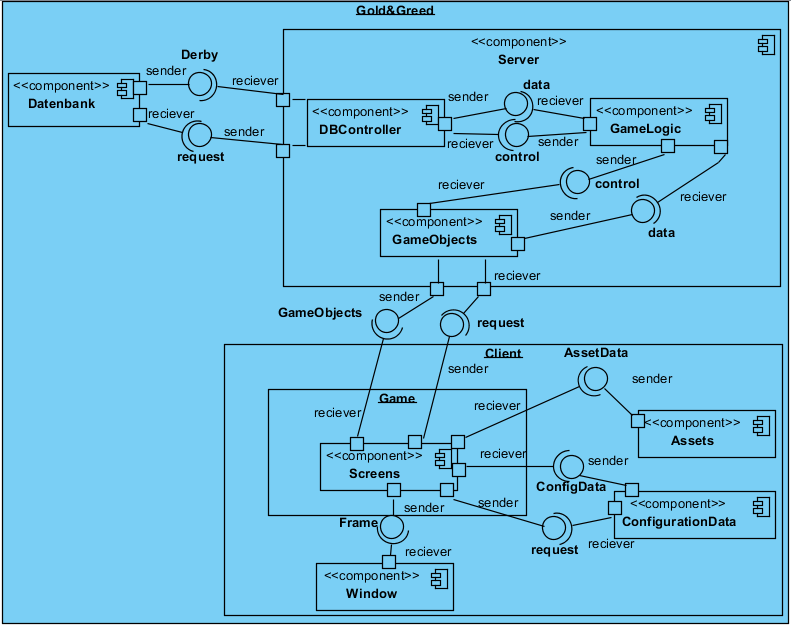
\includegraphics[width=1\linewidth]{ComponentDiagram1}
\caption[Komponenten des Programms]{Die Komponenten des Programms}
\label{fig:ComponentDiagram1}
\end{figure}

\subsection{Datenbank}

Hierbei handelt es sich um eine externe Komponente, welche zwar verwendet, aber nicht selbst implementiert wird. Wobei extern sich hier auf die ablaufenden Prozesse bezieht, die Datenbank selbst ist direkt in das Programm integriert. Die Datenbank kümmert sich um das Speichern von Daten, auch über ein Beenden des Programmes hinaus. Es wird eine Derby Datenbank verwendet. Die Kommunikation mit der Datenbank wird in der Komponente ''DBController'' beschrieben. 

\subsection{Server}

Bei dieser Komponente handelt es sich um eine Sammelkomponente, welche alle Elemente umfasst, die auf dem Server ausgeführt werden. Die Aufgabe der Server-Komponente ist es die Kommunikation zwischen verschiedenen Clients zu ermöglichen und zu verwalten. Außerdem finden hier jegliche darstellungsunabhängige Logikprozesse statt, sowie die Kommunikation mit der Datenbank. 

\subsubsection{DBController}

Diese Komponente stellt die Schnittstelle zwischen Server und Datenbank dar. Sie kommuniziert über Anfragen mit der Datenbank, um Daten zu Speichern oder zu erhalten und an die übrige Logik zurückzugeben. Dabei ist zu beachten, dass der DBController keinen Einfluss darauf nimmt welche Daten, wann gespeichert werden sondern lediglich auf Anfragen aus ''GameLogic'' reagiert.

\subsubsection{GameLogic}

Die GameLogic-Komponente umfasst jegliche darstellungsunabhängige Logik, ausgenommen Datenobjekte. Dies beinhaltet alle Klassen welche nicht mit dem Client geteilt werden. Hier wird außerdem entschieden welche Daten, wann gespeichert oder für welche Clients zur Verfügung gestellt werden. Zum Speichern, bzw. Laden sendet diese Komponente Aufforderungen und entsprechende Daten, bzw. Anfragen an den DBController, welcher dann die Kommunikation mit der Datenbank übernimmt. Die Verbindung zu ''GameObjects'' besteht hauptsächlich aus einem Verwenden der Komponente, wobei spezielle Elemente aus ''GameObjects'' auch Anfragen an die GameLogic senden können.

\subsubsection{GameObjects}

Dies ist das letzte Element innerhalb des Servers. In dieser Komponente befinden sich alle mit dem Client geteilten Objekte, das beinhaltet fast alle darstellbaren Objekte, sowie spezielle Verwaltungsobjekte für den Zugriff auf die ''GameLogic''. Diese Komponente stellt auch die Zugriffsschnittstelle für die Clients zur Verfügung, welche speziell durch Remote-Interfaces innerhalb von GameObjects realisiert wird. Obwohl sich hier die darstellbaren Objekte befinden, besteht hier keine Verbindung zu den Assets, stattdessen findet man hier nur die Information, welche Assets zu einem Objekt gehören, um dann später in ''Screens'' verwendet zu werden.

\subsection{Client}

Beim Client handelt es sich um die Komponente, welche bei jedem Spieler läuft, sie kümmert sich um die Darstellung eines Spiels und lokale Einstellungen.

\subsubsection{Game}

Die Game-Komponente dient lediglich zur Veranschaulichung, dass es sich hierbei um das tatsächliche Programm handelt, ist ansonsten jedoch nur eine Containerkomponente für ''Screens''.

\subsubsection{Screens}

Diese Komponente kommuniziert über die Remote-Interfaces mit ''GameObjects'' und so mit dem Server. Die Komponente fragt alle, für eine grafisch korrekte Darstellung der Spiellogik, relevanten Informationen ab und leitet Spieler-Eingaben weiter. Für die Darstellung greift die Komponente auf ''Assets'' zu, was jedoch in der entsprechenden Komponente erläutert wird. Außerdem werden hier lokale Einstellungen wie Ton-Lautstärke oder Auflösung verwaltet. Dazu weiteres in ''ConfigurationData''. Die tatsächliche Darstellung im Fenster wird vom LibGdx-Framework übernommen.

\subsubsection{Assets}
Hierbei handelt es sich nicht um implementierte Teile des Systems sondern um grafische Dateien, welche auf dem Computer des Clients liegen. Diese Grafiken stellen die verschiedenen Objekte eines Spiels dar(z.B. Einheiten) und werden von ''Screens'' geladen und unter Verwendung des LibGdx-Framework dargestellt. Da diese Darstellung nur für den Client relevant ist, gibt es keine direkte Beziehung zu ''GameObjects'', da dort lediglich Zugehörigkeiten gespeichert werden, jedoch keine Verwendung statt findet.

\subsubsection{ConfigurationData}
Diese Komponente beschreibt ebenfalls nur Dateien und keinen implementierten Teil des Systems. Die Dateien enthalten Client-relevante Informationen, welche in erster Linie von den Präferenzen oder Bedürfnissen des jeweiligen Spielers abhängen. Darunter fallen vor allem Einstellungen bezüglich Darstellung und Ton, sowie ggf. Steuerung. Dabei ist jedoch anzumerken, dass die Einstellungen pro Computer und nicht pro Spieler gespeichert werden. Die Informationen werden dann von der Screens-Komponente verwendet, um ihre Aufgaben präziser zu erfüllen. Das Speichern und Laden der Informationen wird dabei vom LibGdx-Framework umgesetzt.

\subsubsection{Window}

Die Window Komponente beschreibt keine persistenten Elemente des Systems sondern lediglich das am Ende dargestellte Fenster, welches die Schnittstelle zum Spieler realisiert. Die einzelnen Bilder(Frames) werden dabei von den Screens definiert und durch das LibGdx-Framework an das System  weitergegeben, wo dann die endgültige Darstellung des Fensters stattfindet.

\subsection{Bezug zu den Strategien}
Hier wird die Verbindung zwischen den Komponenten und den Strategien erläutert.\\\\
Die Strategie zum Verwenden vom ''RMI'' findet sich in den Komponenten ''GameObjects'' und ''Screens'' wieder, speziell ihrer Kommunikation, welche die in der RMI-Strategie beschriebenen Remote-Interfaces verwendet.. \\

 Die Mindestanforderungen werden hauptsächlich im Server umgesetzt und der Zugriff dann über den Client ermöglicht. \\

Die Strategie ''Don't trust the Client'' findet sich in den Inhalten der Server- und Client-Komponenten, beschrieben in ihren Aufgaben. Verdeutlicht durch die Screens-Komponente, welche die einzige implementierte Komponente in ''Client'' darstellt und entsprechend der Strategie nur Darstellung jedoch keine direkte Logik umsetzt. \\

Im Kommentar zu Anfang des Kapitels ist die Verbindung zu ''Einzelnes Programm'' zu finden. \\ 

Die in ''Aufteilung nur Modul-intern'' beschriebenen Bereiche entsprechenden den hier erläuterten (elementaren) Komponenten. Eine Aufteilung von zu implementierten Teilen findet also nur innerhalb dieser Komponenten statt.\\


\section{Modulsicht}
\label{sec:modulsicht}
Die Modulsicht wird im Groben durch das folgende Paketdiagramm dargestellt, dass Ähnlichkeiten zur konzeptionellen Sicht aufweist. Da wir im Verlauf dieses Kapitels den Inhalt dieser Pakete mit seinen Ports erläutern und diesen beschreibend auf die konzeptionelle Sicht abbilden, nutzen wir Klassendiagramme mit einer Erweiterung durch Ports. Spezifisch zum Aufbau erkennt man hierbei eine Trennung der Assets und Config-Datei vom Client-Paket, wodurch das Data-Paket entstanden ist. Es gibt also vier große Pakete: Der eben erwähnte Client und Data. Derby, dass die Datenbank enthält. Server, mit Spiellogik und der Kommunikation des Servers mit der Datenbank sowie dem Client. Jegliche im folgenden Kapitel genannten Interfaces erweitern die Klasse ''RemoteInterface'' aus der RMI API, um eine Verwendung über RMI zu ermöglichen.

\begin{figure}[h]
\centering
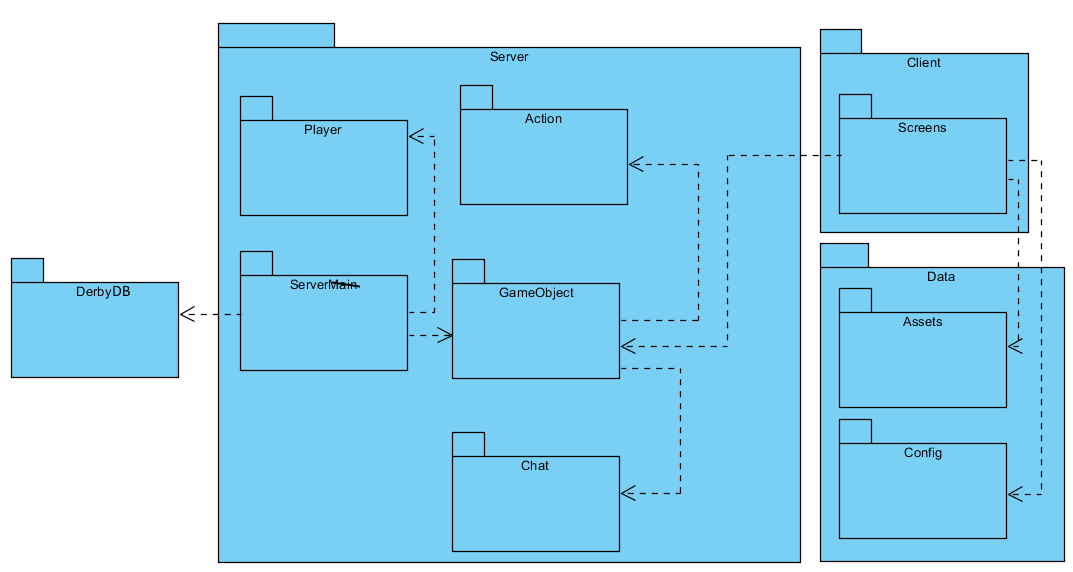
\includegraphics[width=1.0\linewidth]{Paketdiagramm}
\caption{Ein Paketdiagramm das eine grobe Modulsicht und ihre Importbeziehungen zeigt.}
\label{fig:Paketdiagramm}
\end{figure}

\subsection{Server-Modul}

Das Server-Modul beinhaltet die Server-Klasse sowie den DBManager. Es stellt also eine Überschneidung der DBController-Komponente und GameLogic-Komponente dar. Seine Aufgabe ist einerseits die Kommunikation mit der Datenbank und andererseits den initialen Zugriff auf den Server-Computer zu ermöglichen.

\begin{figure}[h]
\centering
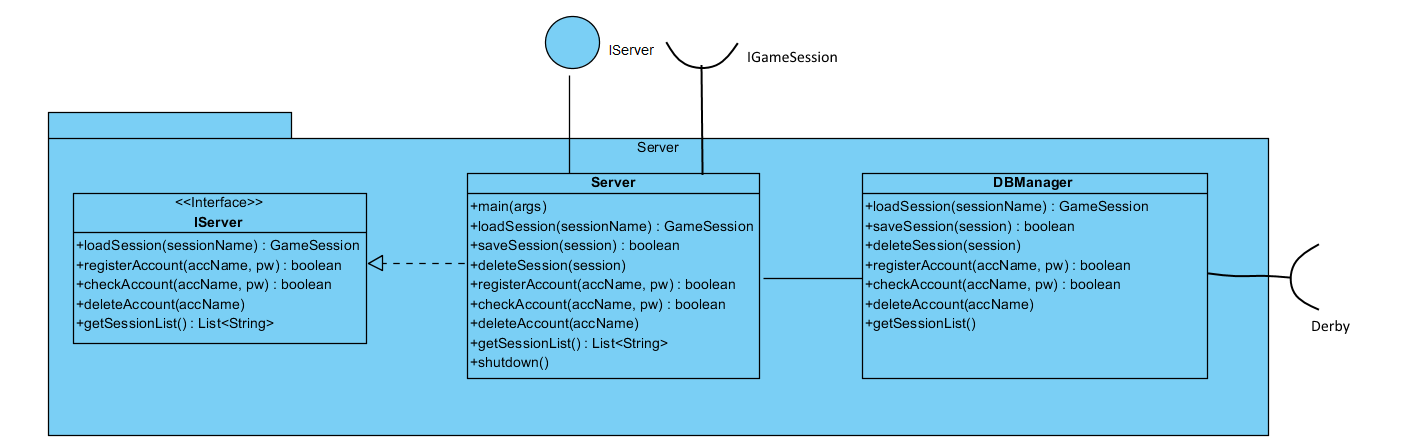
\includegraphics[width=1.0\linewidth]{ServerClass}
\caption{Das Server-Package als Klassendiagramm}
\label{fig:ServerClass}
\end{figure}

Die Klasse Server besitzt eine main-Methode, da sie nicht nur den initialen Zugriff auf den Server ermöglicht sondern auch das zugrundeliegende Programm initialisiert. Beim initialisieren erstellt die Klasse eine neue Registry auf dem Computer und registriert sich selbst, um so den Zugriff über RMI zu ermöglichen. Ist bereits eine Registry vorhanden, wird diese verwendet. Die Registry wird in einem statischen Attribut ermöglicht, wodurch der Server nicht automatisch beendet wird, da die Registry nicht vom Garbage-Collector eingesammelt wird. Ansonsten ist vor allem die getSessionList()-Methode interessant, diese liefert eine Auswahl von allen verfügbaren Spielen und dient so als Ausgangspunkt zum Laden eines Spiels.

Das Interface IServer besitzt alle für den Client relevanten Methoden und ist die für RMI eigentlich verwendete Komponente, also die initiale Schnittstelle nach außen.

Die Klasse DBManager besitzt nur eine erhaltende Schnittstelle, welche von Derby bereit gestellt wird. Ansonsten besteht nur eine Verbindung zu Server, da Server den DBManager für die Kommunikation mit der Datenbank verwendet.

\subsection{Chat}

Das Chat-Modul besitzt die Aufgabe jegliche Nachrichtensysteme umzusetzen, bisher umfasst dies nur die Klassen Chat und Message. Es ist eines der drei Module welche zusammen die GameObject-Komponente darstellen, die anderen beiden sind Player und GameObject.

\begin{figure}[h]
\centering
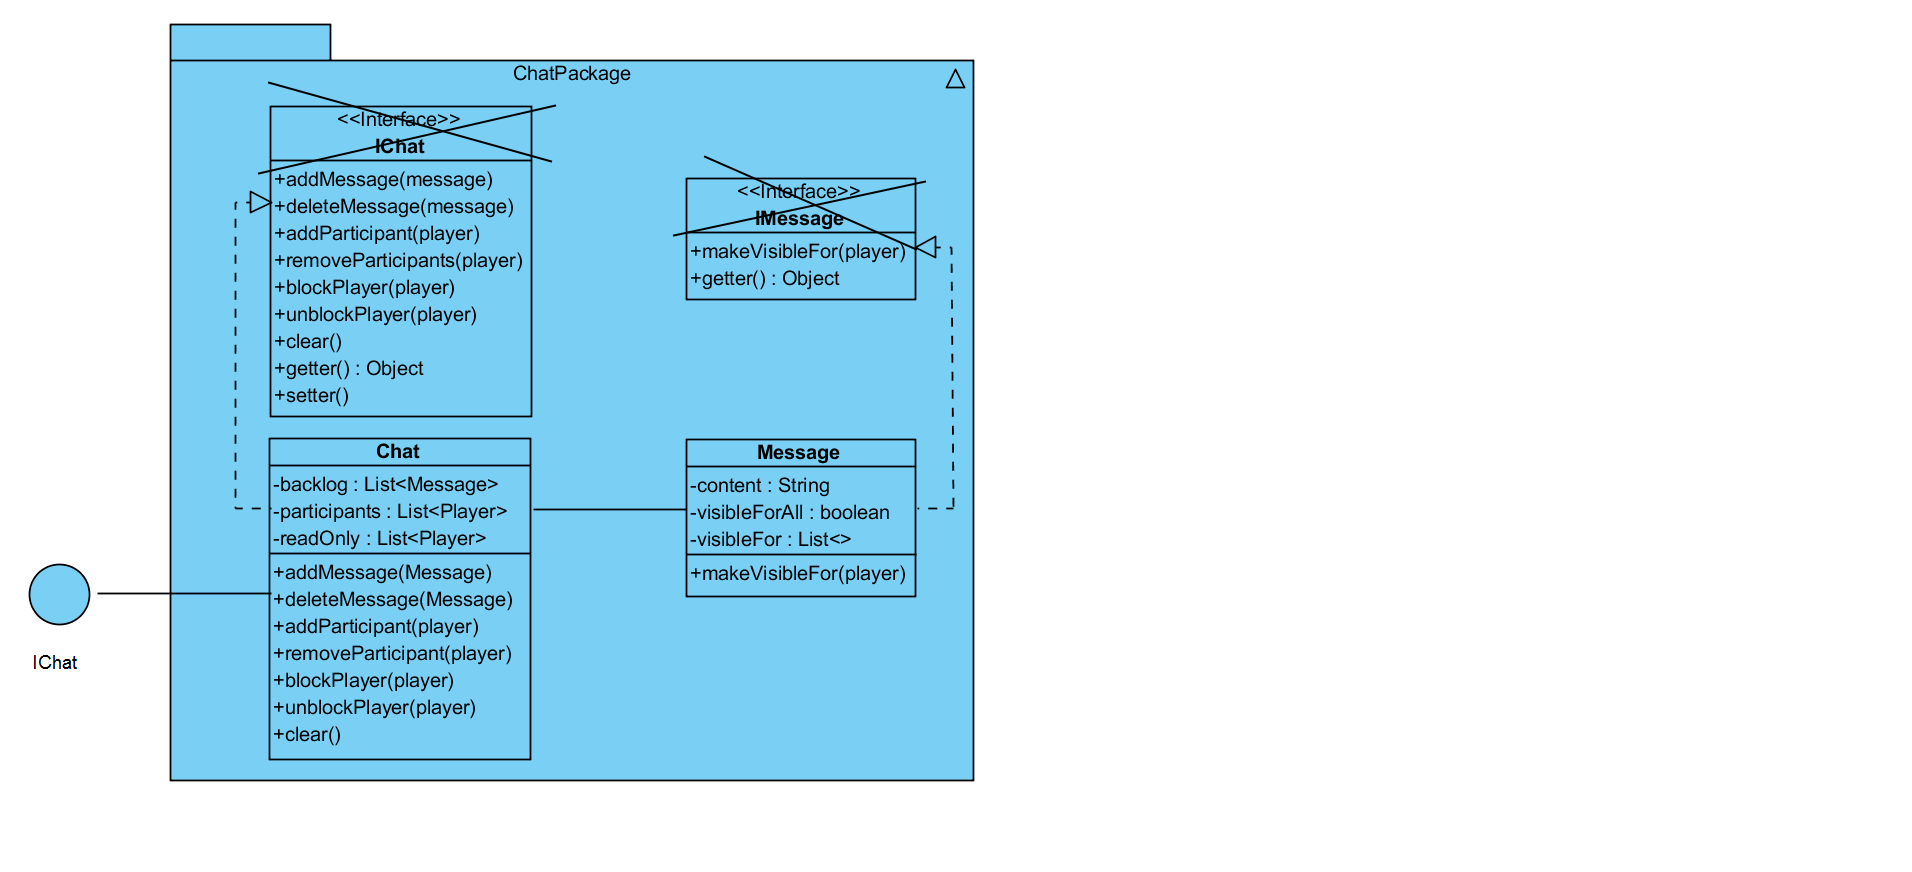
\includegraphics[width=1.0\linewidth]{ChatClass}
\caption{Das Chat-Modul als Klassendiagramm}
\label{fig:ChatClass}
\end{figure}

Die Message-Klasse beschreibt eine einzelne Nachricht innerhalb eines Chats. Dies wurde als eigene Klasse realisiert, um zusätzliche Funktionen wie das Ausschließen von Spielern zu vereinfachen, weitere Funktionen sind bisher nicht vorhanden.

Der Kern des Chat-Moduls ist jedoch die Chat Klasse, welche eine Sammlung von Nachrichten ist und Informationen darüber besitzt, wer am Chat mit welchen Rechten teilnimmt.

Beide Klassen besitzen Interfaces, um ihre Verwendung auch vom Client aus zu ermöglichen. Die Interfaces besitzen dabei auch die getter-Methoden um sie dem Client zur Verfügung zu stellen. Da diese Methoden jedoch trivial sind und sich durch die Attribute in der implementierenden Klasse definieren, wurden sie unter dem Punkt getter zusammengefasst mit Object als Rückgabetyp. 

Obwohl die Klassen durch ihre Interfaces direkt vom Client zugegriffen werden könnten, ist die Schnittstelle hauptsächlich für GameSession aus GameObjects als direkten Zugriff gedacht und stellt für den Client lediglich die Funktionalität zur Verfügung. Weiteres zum Zugriff in GameObjects.

\subsection{GameObject}

Das GameObject-Modul ist der größte Teil aus der GameObjects-Komponente und gewissermaßen ihr Kern. Es beinhaltet jegliche Klassen, welche am Ende in einer Spielsession dargestellt und verwendet werden sowie das Objekt für die Spielsession selbst(GameSession). Ausgenommen davon sind die Chat-Objekte, da das Nachrichtensystem als eigenes Modul betrachtet wird und jegliche Spieler-bezogenen Objekte, welche nicht direkt (grafisch) dargestellt werden, sich im Player-Modul befinden. Die Aufgabe des Moduls ist es dem Client weiteren Zugriff, nach dem initialen Zugriff zu ermöglichen und seine Anfragen mit den Spiel-Objekten sowie der Spielelogik zu verbinden.

\begin{figure}[h]
\centering
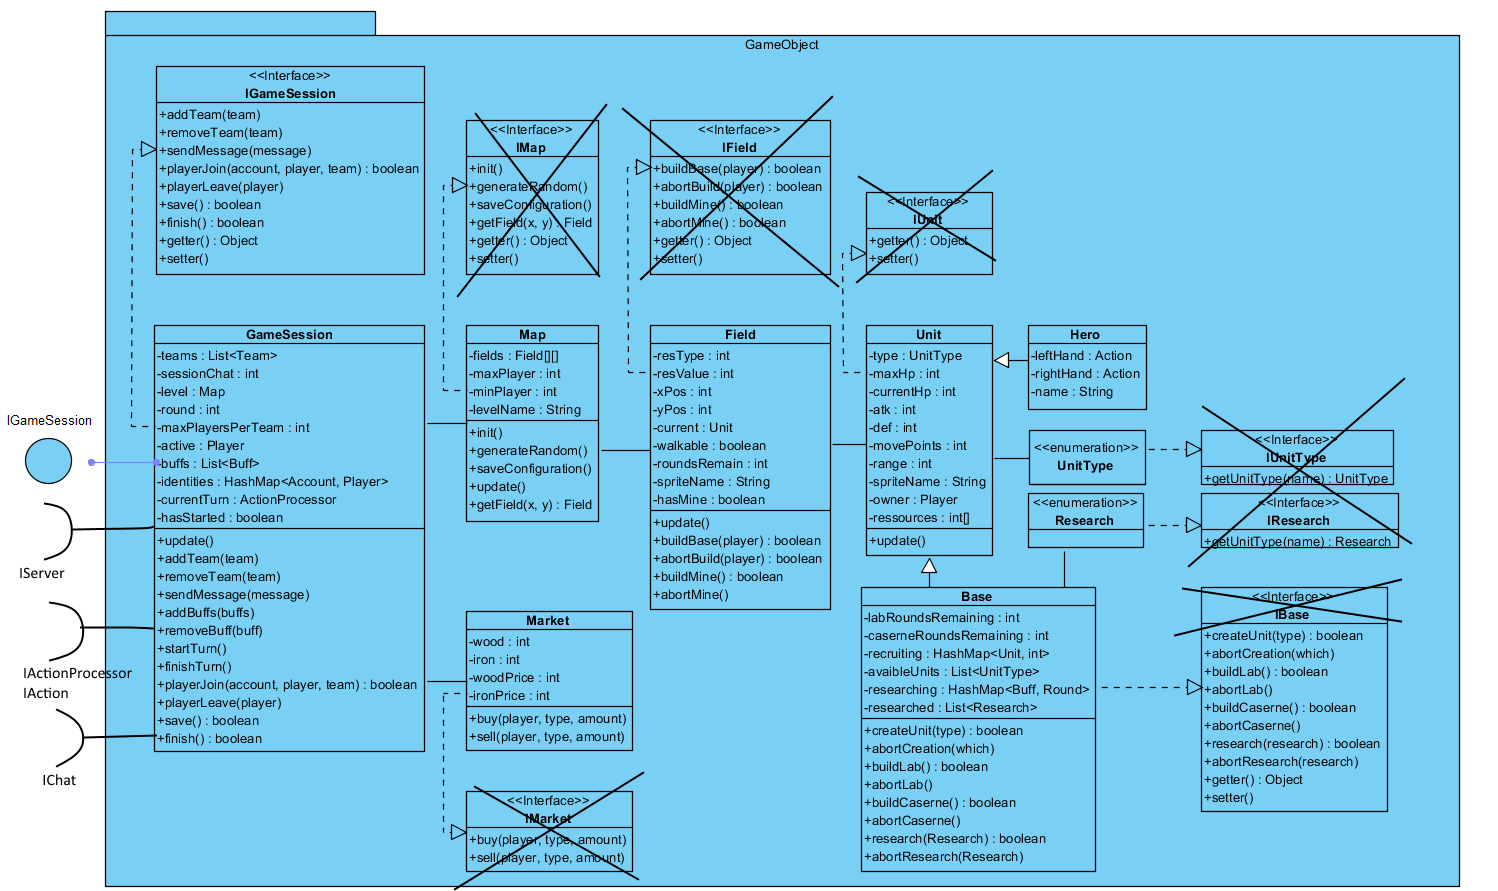
\includegraphics[width=1.0\linewidth]{GameObjectsClass}
\caption{Das GameObjects-Modul als Klassendiagramm}
\label{fig:GameObjectsClass}
\end{figure}

Jegliche Klassen in diesem Modul besitzen Interfaces, um ihre Funktionalität dem Client zur Verfügung zu stellen, dabei beinhalten sie nur die Methoden, welche auch für den Client relevant sind. Updates werden z.B. von GameSession übernommen, weshalb entsprechende Methoden nicht für den Client zugänglich sind. Dafür besitzen sie getter-Methoden, welche auch hier allgemein abgekürzt wurden, mit Object als Rückgabewert, weil sie wieder trivial sind und sich durch die Attribute in der implementierenden Klasse definieren. Die Objekte dieses Moduls realisieren die meisten der Mindestanforderungen, ausgenommen sind dabei vor allem der Datenbank-Teil sowie die Server-Client Struktur.

Auch die beiden Enumerations, UnitType und Research besitzen Interfaces, welche lediglich eine get-Methode besitzen. Diese ermöglicht dem Client den gewünschten Enumwert zu einem String zu erhalten.

Obwohl die Interfaces die Verwendung aller Objekte durch den Client ermöglichen und so Teil der Schnittstelle zwischen der Screens und GameObjects-Komponente sind, dienen sie nur zur Bereitstellung der Funktionalität. Der Zugriff wird über GameSession geregelt.

Daher stellt GameSession den Kern diese Moduls dar. Da sie alle Objekte einer Spielsession besitzt, greift der Client auf die GameSession zu und erhält so auch Zugriff auf die anderen Objekte. Zusammen stellen die Interfaces also die Schnittstelle zwischen den Komponenten, Screens und GameObjects dar. Neben der Verbindung zu Screens, verwendet GameSession auch Server aus dem Server-Modul und Action aus dem Action-Modul, welche sich beide in der GameLogic-Komponente befinden. Die Verwendung zwischen Server und GameSession ist dabei beidseitig. Somit stellt GameSession also beide Schnittstellen der GameObject-Komponente dar, einerseits die zu Screens, andererseits jedoch auch die zwischen GameObjects und GameLogic.

\subsection{Action}
Das Action-Modul beinhaltet vor allem Logik, die auf die Interaktion zwischen Spielobjekten bezogen ist. Das umfasst die Action-Klassen, sowie den ActionProcessor. Der Zugriff erfolgt auch hier über die entsprechenden Interfaces. Die Klasse ist Teil der GameLogic-Komponente.

\begin{figure}[h]
\centering
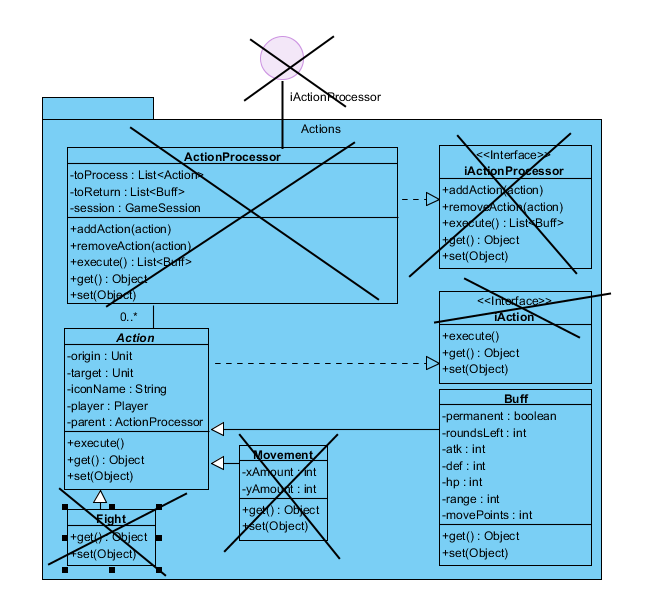
\includegraphics[width=1.0\linewidth]{ActionClass}
\caption{Das Action-Modul als Klassendiagramm}
\label{fig:ActionClass}
\end{figure}

Der ActionProcessor ist die Schnittstelle des Moduls nach außen. Er besitzt Listen mit den zu verarbeitenden Objekten und Buff-Objekten, welche möglicherweise beim Verarbeiten der Actions generiert wurden. Der ActionProcessor wird dabei von GameSession für je einen Zug verwendet. Beendet ein Spieler seinen Zug wird der ActionProcessor angewiesen alle ihm zugeordneten Actions zu verarbeiten, dafür dient die execute-Methode. Sollten bei diesem Prozess Buffs entstehen werden diese am Ende als Liste zurückgegeben, um in GameSession gespeichert werden zu können.

Die zweite besonders wichtige Klasse ist Action. Diese Klasse beschreibt eine ausführbare Aktion, welche in der Regel zwei Teilnehmer besitzt, wobei es auch nur einen Teilnehmer geben kann. Die Action kann über ihre execute-Methode ausgeführt werden, wobei der Inhalt dieser Methoden von der speziellen Implementierung abhängt. Beispiele dafür sind die bereits definierten Actions Movement und Fight, welche eine Bewegung und einen Kampf realisieren, bisher sind keine weiteren Actions geplant.

Zuletzt ist noch die Buff-Klasse zu sehen. Dies ist eine spezielle Action, welche nach ihrem Ausführen nicht sofort verworfen wird und sogar permanent aktiv sein kann. Sie besitzt Attribute ähnlich zu denen von Einheiten. Die Werte dieser Attribute bestimmen, wie die Werte der Einheiten manipuliert werden. Dazu mehr im nächsten Kapitel. 

\subsection{Player}
Das Player-Modul ist das letzte Modul der GameObjects-Komponente. Es umfasst alle Klassen, welche direkt Spieler bezogen sind und somit nur indirekt auf dem Spielfeld dargestellt werden (z.B. Farbe von Einheiten). Auch hier erfolgt der Zugriff von außen über die Interfaces.

\begin{figure}[h]
\centering
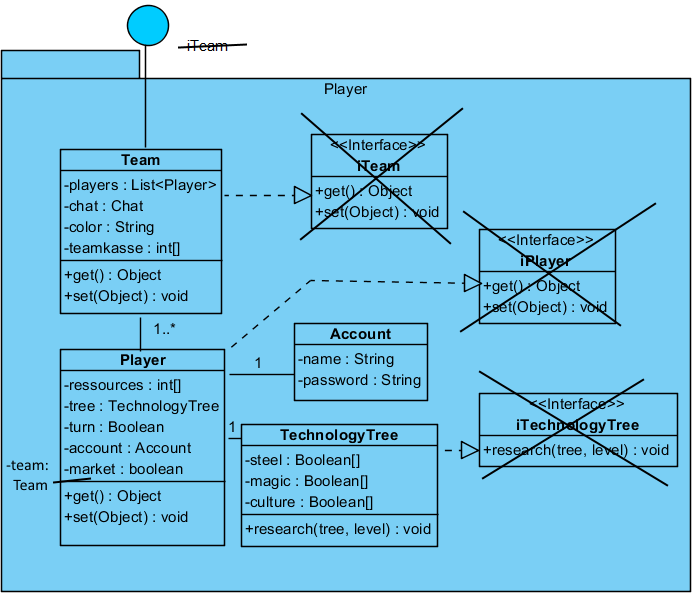
\includegraphics[width=1.0\linewidth]{PlayerClass}
\caption{Das Action-Modul als Klassendiagramm}
\label{fig:PlayerClass}
\end{figure}

Die Schnittstelle nach außen stellt hier die Teamklasse dar, da eine GameSession zwar die teilnehmenden Spieler kennt, das Spiel an sich aber über die Teams verwaltet wird. Sollte es nur zwei Spieler geben, gibt es dementsprechend zwei Teams mit je einem Spieler. Ein Team besitzt eine Liste mit allen Mitgliedern, einen Chat und eine Teamfarbe. Außerdem wird auch die in den Mindestanforderungen geforderte Teamklasse hier umgesetzt. Genaueres dazu findet sich in der Datensicht. 

Neben dem Team beinhaltet das Modul auch die Playerklasse selbst. Diese stellt einen Spieler innerhalb einer Spielsitzung dar. Es ist also das Referenzobjekt, wenn geprüft wird, zu wem eine Einheit gehört. Dafür besitzt der Spieler außerdem das TechnologyTree-Objekt, welches darstellt, welche Technologien der Spieler bereits erreicht hat. Die Technologien beziehen sich dabei auf Aufwertungen, die den Spieler direkt betreffen, Forschungen bezüglich Einheiten werden in Basen, genauer dem Laboratorium verwaltet.

Zuletzt beinhaltet das Modul das Account-Objekt. Dieses Identifiziert einen Spieler auch über eine Spielsitzung hinaus und wird verwendet um z.B. beim Laden eines Spiels die Player korrekt den Teilnehmern zuzuordnen. Bisher beinhaltet diese Klasse keine weiteren Informationen, es wäre jedoch denkbar, die Klasse um zusätzliche Statistiken, wie z.B. Sieg-Niederlage Verhältnis zu erweitern. Um diese Möglichkeit nicht auszuschließen wurde der Account als Objekt umgesetzt, ansonsten hätte man auch direkt den Accountnamen in Player speichern können.

\subsection{Screens}
Zuletzt haben wir noch das Screens-Modul, welches die Screens-Komponente beschreibt. Alle Klassen in diesem Modul sind Unterklassen von AbstractGameScreen und dienen zur Darstellung verschiedener Bildschirme. Dieses Modul besitzt keine Interfaces, da es nur auf andere Objekte zugreift, selbst aber nicht zugegriffen wird, da die Darstellung die höchste Instanz bezüglich der Aufrufhierarchie des Programms ist.

\begin{figure}[h]
\centering
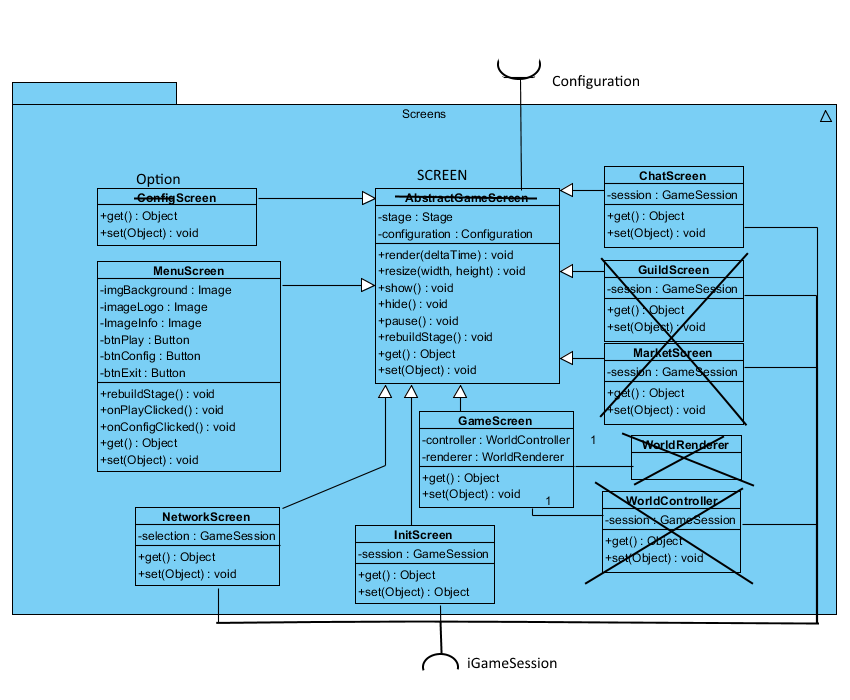
\includegraphics[width=1.0\linewidth]{ScreenClass}
\caption{Das Screens-Modul als Klassendiagramm}
\label{fig:ScreenClass}
\end{figure}

Der Kern des Moduls ist wie bereits genannt die Klasse AbstractGameScreen. Sie beschreibt welche Methoden und Attribute von allen Screens implementiert werden müssen, diese Ergeben sich durch das libGdx-Framework, wobei es sich dabei Teilweise nur um Konventionen handelt. Die Methoden und Attribute befassen sich dabei hauptsächlich mit der Darstellung der Bildschirme.

Die anderen Klassen implementieren diese Methoden dann lediglich mit den für den jeweiligen Bildschirm relevanten Informationen, weshalb sie hier nicht weiter erläutert werden, stattdessen folgt eine kurze Beschreibung der Screens und eine Auflistung der benötigten Funktionen:

\begin{itemize}
\item \textbf{ConfigScreen:} In diesem Bildschirm können die Werte für das Configuration Objekt eingestellt werden. \\ Benötigte Funktionen:
\begin{itemize}
\item \textbf{Einstellen der Auflösung}
\item \textbf{Einstellen der Lautstärke}
\item \textbf{Musik deaktivieren/aktivieren}
\item \textbf{Zu MenuScreen navigieren}
\end{itemize}

\item \textbf{MenuScreen:}Dieser Bildschirm stellt das Hauptmenü dar und ist der initiale Bildschirm nach dem Start. \\ Benötigte Funktionen:
\begin{itemize}
	\item \textbf{Wechseln zu ''NetworkScreen''}
	\item \textbf{Wechseln zu ''ConfigScreen''}
	\item \textbf{Beenden des Spiels}
	\item \textbf{Registrieren von neuem Account}
\end{itemize} 

\item \textbf{NetworkScreen:} Der NetworkScreen liefert eine Liste mit allen verfügbaren Spielen, sowie die Möglichkeit ein neues Spiel zu erstellen.\\ Benötigte Funktionen:
\begin{itemize}
	\item \textbf{Einloggen in Account.}
	\item \textbf{Wechseln zu ''MenuScreen''.}
	\item \textbf{Auswählen eines existenten Spiels zum Beitreten bzw. Laden.} Führt zu ''InitScreen'', wobei das ausgewählte Spiel übergeben wird.
	\item \textbf{Erstellen eines neuen Spiels.} Führt zu ''InitScreen'', ohne das ein Spiel übergeben wird.
\end{itemize}

\item \textbf{InitScreen:}
Dieser Screen liefert einen Überblick über die Einstellungen des Spiels und ermöglicht es sie zu bearbeiten sofern das Spiel neu erstellt wird.\\ Benötigte Funktionen:
\begin{itemize}
	\item \textbf{Zurückkehren zu ''NetworkScreen''.}
	\item \textbf{Auswählen eines Teams.}
	\item \textbf{Minimale und maximale (pro Team) Spieleranzahl angeben.} Host exklusiv.
	\item \textbf{Auswählen der Spielmap.} Host exklusiv.
	\item \textbf{Spiel starten.} Host exklusiv.
\end{itemize}

\item \textbf{GameScreen:}
Hier wird das laufende Spiel dargestellt. Um eine einwandfreie Darstellung zu gewährleisten, sollen hier die Hilfsklassen ''WorldController'' und ''WorldRenderer'' verwendet werden, daher werden diese als Attribute gespeichert.\\ Benötigte Funktionen:
\begin{itemize}
	\item \textbf{Alle in den Mindestanforderungen genannten Möglichkeiten eines Spielers innerhalb eines laufenden Spiels.} Details: Siehe Mindestanforderungen.
\end{itemize}

\item \textbf{MarketScreen:}
In diesem Bildschirm wird der Marktplatz eines Spiels dargestellt.\\ Benötigte Funktionen:
\begin{itemize}
	\item \textbf{Kaufen/Verkaufen von Holz.}
	\item \textbf{Kaufen/Verkaufen von Eisen.}
	\item \textbf{Zurückkehren zum GameScreen.}
\end{itemize}

\item \textbf{GuildScreen:}
Hier werden Teamrelevante Informationen angezeigt und Funktionen zur Verfügung gestellt.\\ Benötigte Funktionen:
\begin{itemize}
	\item \textbf{Teamnachrichten schreiben und lesen.}
	\item \textbf{In die Teamkasse einzahlen und Kassenstand betrachten.}
	\item \textbf{Zurückkehren zum GameScreen.}
\end{itemize}

\item \textbf{ChatScreen:}
Hier erhält der Spieler Zugriff auf seine Chatunterhaltungen.\\ Benötigte Funktionen:
\begin{itemize}
	\item \textbf{Zurückkehren zum vorherigen Screen.}
	\item \textbf{Nachrichten in einem Chat schreiben und lesen.}
\end{itemize}
\end{itemize}


Die eingehende Schnittstelle von IGameSession verweist zwar auf InitScreen, jedoch ist dies lediglich die initiale Verbindung, das GameSession-Objekt wird dann an die anderen Screens weiter gegeben und dort ebenfalls durch das Remote-Interface von GameSession weiter verwendet.

Die Configuration und Assets werden dabei direkt aus den jeweiligen Dateien geladen, wobei libGdx zur Hilfe verwendet wird.

\section{Datensicht}
\label{sec:datensicht}

Für eine bessere Übersicht wurden die Interfaces in diesem Diagramm weg gelassen, da sie ohnehin nur für die Verwendung von RMI benötigt werden.

\begin{figure}[h]
\centering
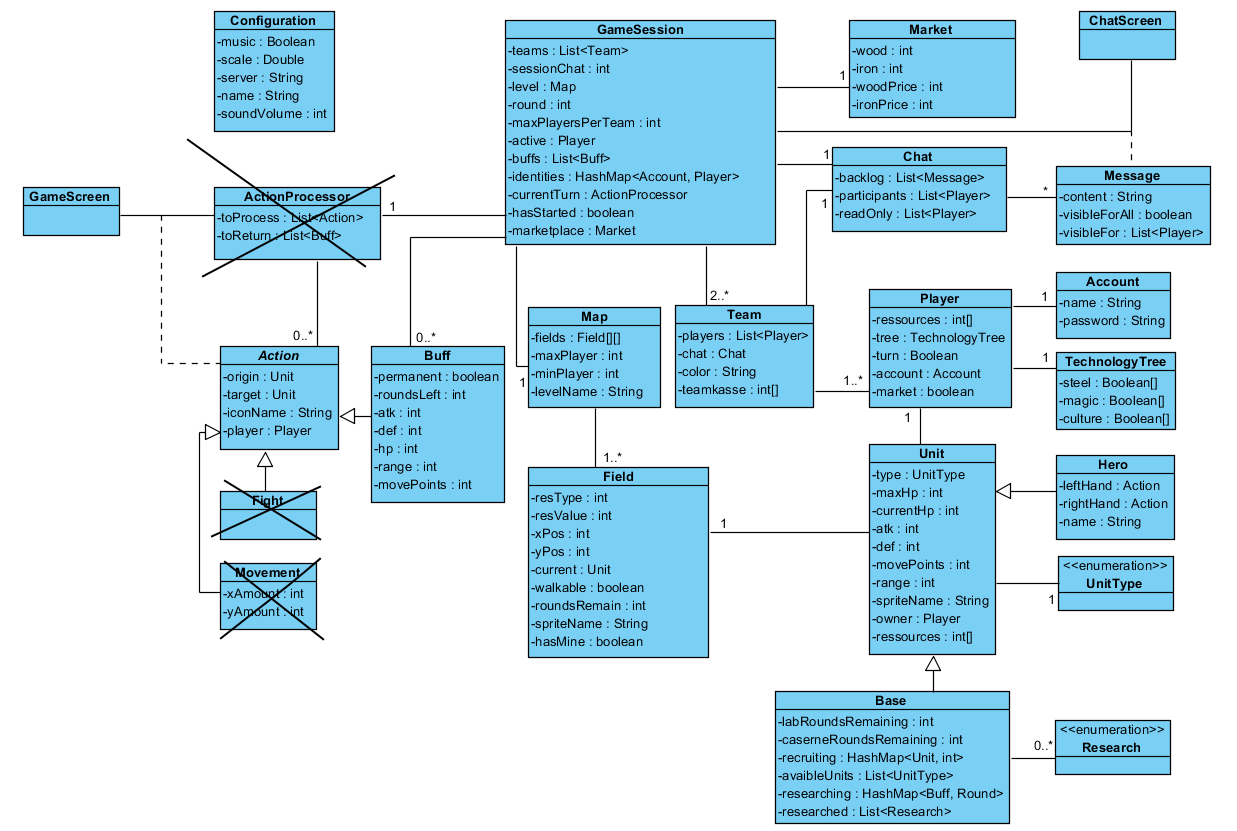
\includegraphics[width=1.0\linewidth]{DatensichtForReal}
\caption{Die Datenklassen von Gold and Greed}
\label{fig:ClassDiagram1}
\end{figure}

\subsection{Client}

\subsubsection{MainGame}

Diese Klasse dient lediglich zum Initialisieren des Clients und besitzt daher nur die allgemein bekannte Methode ''void main(String args[])''. In dieser Methode wird dann die Verbindung zum Server aufgebaut und der erste Bildschirm(MenuScreen) initialisiert.

\subsubsection{Configuration}
Diese Objekt dient zum Speichern und Laden von lokalen Einstellungen wie z.B. Auflösung oder Lautstärke von Ton. Die Einstellungen werden durch das Framework automatisch auf dem Computer gespeichert und geladen.

\textbf{Attribute:}
\begin{itemize}
	\item \textbf{music:} Bestimmt ob Musik gespielt werden soll oder nicht.
	\item \textbf{scale:} Bestimmt die Skalierung aller dargestellten Elemente.
	\item \textbf{server:} Beinhaltet eine Liste mit allen zur Verfügung stehenden Servern.
	\item \textbf{soundVolume:} Gibt die Lautstärke aller Töne an. 
\end{itemize}

\subsection{Server}

\subsubsection{GameSession}

Diese Klasse realisiert das zentralste Objekt des Programms, eine Spielesitzung. Sie dient dazu alle in einem Spiel existenten Objekt zu verwalten und ihren Zugriff zu ermöglichen. Hier wird außerdem bestimmt, wann welche Informationen gespeichert werden und die nicht geteilten Spielobjekte verwaltet. \\

\textbf{Attribute:}
\begin{itemize}
\item \textbf{teams:} Eine Liste mit allen Teams des Spiels.
\item \textbf{sessionChat:} Der globale Chat des Spiels.
\item \textbf{level:} Die Karte auf der gespielt wird.
\item \textbf{round:} Die Nummer der aktuellen Runde.
\item \textbf{maxPlayersPerTeam:} Gibt an, wie viele Spieler in einem Team maximal sein dürfen.
\item \textbf{active:} Der Spieler, welcher am Zug ist.
\item \textbf{buffs:} Eine Liste mit allen im Spiel aktiven Buffs, Zuordnung findet zu Spielobjekten findet innerhalb von ''Buff'' statt.
\item \textbf{identities:} Eine HashMap, welche jedem Account einen Spieler zuordnet. Fürs Laden eines Spiels relevant.
\item \textbf{currentTurn:} Ein ActionProcessor, welcher alle Aktionen des aktuellen Zugs verwaltet.
\item \textbf{hasStarted:} Gibt an, ob das Spiel noch Konfiguriert wird oder schon gestartet ist.
\end{itemize}

\subsubsection{ActionProcessor}

In dieser Klasse werden die in einem Zug gegebenen Befehle verarbeitet und umgesetzt.

\textbf{Attribute:}
\begin{itemize}
\item \textbf{toProcess:} Eine Liste mit allen Befehlen(Actions) die in dem aktuellen Zug gegeben werden.
\item \textbf{toReturn:} Eine Liste mit Buffs die beim Verarbeiten der Befehle generiert wurden. Wird später an GameSession zurückgegeben.
\item \textbf{session:} Eine Referenz auf die GameSession, welche dem ActionProcessor gehört, als Zugriffsmöglichkeit.
\end{itemize}

\subsubsection{Action}

Eine abstrakte Klasse für alle Arten von Aktionen. Sie kann von GameScreen erstellt und an den ActionProcessor übergeben werden, ein solcher Prozess findet z.B. bei Usereingaben statt.

\textbf{Attribute:}
\begin{itemize}
\item \textbf{origin:} Die Einheit von der die Aktion ausgeht, bzw. auf der sie ausgeführt. Z.B. die zu bewegende Einheit.
\item \textbf{target:} Die Zieleinheit, sofern es eine gibt. Z.B. die angegriffene Einheit.
\item \textbf{iconName:} Gibt den Namen des Iconsprites zur Darstellung auf dem Client an.
\item \textbf{player:} Der Spieler für den die Aktion gilt. Relevant sofern es direkte Auswirkungen auf einen Spieler und nicht auf seine Einheiten hat.
\item \textbf{parent:} Der ActionProcessor, der diese Action verwaltet, als Zugriffspunkt. Bei Buffs null.
\end{itemize}

\subsubsection{Fight}

Eine Implementation einer Action zum Umsetzen eines Kampfes zwischen ''Origin'' und ''Target''.

\textbf{Attribute:}
Keine speziellen.

\subsubsection{Movement}

Eine Implementation einer Action zum Bewegen von Einheiten(''Origin'').

\textbf{Attribute:}
\begin{itemize}
\item \textbf{xAmount:} Gibt an wie viele Felder in X-Richtung gegangen werden sollen. Orientierung wird durch positive und negative Werte realisiert.
\item \textbf{yAmount:} Gibt an wie viele Felder in Y-Richtung gegangen werden sollen. Orientierung wird durch positive und negative Werte realisiert.
\end{itemize}

\subsubsection{Buff}

Ein Buff ist eine spezielle Form einer Action, mit der Eigenschaft, dass sie nicht nur einmal ausgeführt wird sondern mehrfach. Ihre Aktion besteht aus dem Manipulieren von Einheiten Werten.

\textbf{Attribute:}
\begin{itemize}
\item \textbf{permanent:} Gibt an, ob es sich bei dem Buff um eine dauerhafte Verbesserung handelt oder eine Temporäre.
\item \textbf{roundsLeft:} Gibt an, wie viele Runden der Buff noch aktiv bleibt. Falls ''permanent'' \textbf{true} ist, ist dieser Wert -1. Ist dieser Wert 0, löscht sich der Buff selbst beim nächsten Update(execute).
\item \textbf{atk:} Dieser Wert wird auf den gleichnamigen Wert der ''target'' Einheit einmalig addiert. Löscht sich der Buff wird der Wert wieder subtrahiert. Der Wert darf negativ sein und so Minderungen darstellen.
\item \textbf{def:} Analog zu atk.
\item \textbf{hp:} Analog zu atk. Bezieht sich auf ''maxHp''
\item \textbf{range:} Analog zu atk.
\item \textbf{movePoints:} Analog zu atk.
\end{itemize}

\subsubsection{Market}

Über das Marktobjekt können Spieler handeln, wobei man nicht direkt mit anderen Spielern handeln kann.

\textbf{Attribute:}
\begin{itemize}
\item \textbf{wood:} Die Menge an Holz die auf dem Markt verfügbar ist. Erhöht sich wenn Holz verkauft wird.
\item \textbf{iron:} Analog zu ''wood'' für Eisen.
\item \textbf{woodPrice:} Gibt an, wie viel Gold man für das Verkaufen von Holz erhält oder für das Kaufen verliert. Preis ist pro 1 Holz angegeben und wird bei Aufruf von ''buy'' oder ''sell'' neu generiert.
\item \textbf{ironPrice:} Analog zu ''woodPrice'' für Eisen.
\end{itemize}

\subsubsection{Chat}

Ein Chat ermöglicht das Kommunizieren zwischen Spieler über Textnachrichten.

\textbf{Attribute:}
\begin{itemize}
\item \textbf{backlog:} Eine Liste mit allen bisher gesendeten Nachrichten.
\item \textbf{participants:} Alle Spieler die an dem Chat teilnehmen und somit Lesen und Schreiben können.
\item \textbf{readOnly:} Eine Liste mit allen Spielern, die zwar die Nachrichten lesen dürfen, aber keine Schreiben(z.B. weil sie andere beleidigen).
\end{itemize}

\subsubsection{Message}

Eine Message ist eine Chatnachricht, welche jedoch Information über ihre Sichtbarkeit besitzt. Sie kann von ChatScreen erstellt und an GameSession übergeben werden.

\textbf{Attribute:}
\begin{itemize}
\item \textbf{content:} Der Inhalt der Nachricht, welcher im Chat angezeigt wird, als Zeichenkette.
\item \textbf{visibleForAll:} Gibt an, ob jeder diese Nachricht lesen kann. 
\item \textbf{visibleFor:} Falls ''visibleForAll'' \textbf{false} ist, werden in dieser Liste alle Spieler gespeichert, welche die Nachricht lesen dürfen.
\end{itemize}

\subsubsection{Team:}

Ein Team ist eine verbündete Menge von Spielern in einer Sitzung. Damit ein Spiel gewonnen werden kann ist es ausreichend, dass alle übrigen Spieler dem gleichen Team angehören, es muss also keinen einzelnen Sieger geben.

\textbf{Attribute:}
\begin{itemize}
\item \textbf{players:} Eine Liste mit allen Mitgliedern des Teams.
\item \textbf{chat:} Ein Chat der nur für das Team sichtbar ist.
\item \textbf{color:} Die Teamfarbe, Haupterkennungsmerkmal für Teams.
\item \textbf{teamkasse:} Die gemeinsame Kasse des Teams. Verliert ein Teammitglied eine Einheit erhält er einen Teil der Kosten aus dieser Kasse zurück, sofern genug vorhanden sind. Die Werte werden dabei direkt gespeichert und über ihren Index den Ressourcen zugeordnet (0=Holz,1=Eisen,2=Gold). Mana kann nicht zurückgewonnen werden.
\end{itemize}

\subsubsection{Player}
Ein Player ist die Repräsentation eines Accounts innerhalb einer Spielsitzung, also des agierenden Spielers.

\textbf{Attribute:}
\begin{itemize}
\item \textbf{ressources:} Die Ressourcen über die der Spieler verfügt. Die Menge wird direkt als Wert gespeichert und der Typ über den Index identifiziert(0=Holz,1=Eisen,2=Gold,3=Mana).
\item \textbf{tree:} Der TechnologyTree des Spielers, welcher angibt, welche Technologien ein Spieler bereits entwickelt hat.
\item \textbf{turn:} Gibt an ob der Spieler am Zug ist.
\item \textbf{account:} Der zum Spieler gehörende Account.
\item \textbf{market:} Gibt an, ob der Spieler bereits Zugriff auf den Marktplatz hat.
\end{itemize}

\subsubsection{Account}
Die eindeutige Identifikation eines Spielers, auch über Spielsitzungen hinaus. Kann eventuell mit optionalen Werten erweitert werden (z.B. Statistiken über Sieg-Niederlage Verhältnis).

\textbf{Attribute:}
\begin{itemize}
\item \textbf{name:} Der Name des Accounts.
\item \textbf{password:} Das Passwort des Accounts, genauer der Vergleichswert. Wird bei genug übriger Zeit des Projektes zu einem Hash geändert, um so die Sicherheit zu erhöhen.
\end{itemize}

\subsubsection{TechnologyTree}

Ein Technologie-Baum gibt an welche Technologien ein Spieler entwickelt hat.

\textbf{Attribute:}
\begin{itemize}
\item \textbf{steel:} Realisiert den Zweig für Holz und Eisen Erweiterungen. Jede Erweiterung wird durch einen Boolean-Wert dargestellt.
\item \textbf{magic:} Analog zu ''steel'' für Mana-bezogene Erweiterungen.
\item \textbf{culture:} Analog zu ''steel'' für Gold-bezogene Erweiterungen. Hier kann auch der Zugriff auf den Marktplatz freigeschaltet werden. 
\end{itemize}

\subsubsection{Map}

Eine Map stellt ein Level bzw. eine Karte für eine Spielsitzung dar. Hier werden auch alle Felder der Karte gespeichert.

\textbf{Attribute:}
\begin{itemize}
\item \textbf{fields:} Ein X*Y großes Array, welches die einzelnen Spielfelder beinhaltet.
\item \textbf{maxPlayer:} Die maximale Spieler-Anzahl für diese Karte.
\item \textbf{minPayer:} Die minimale Spieler-Anzahl für diese Karte.
\item \textbf{levelName:} Der Name der Karte.
\end{itemize}

\subsubsection{Field}
Ein Feld ist ein einzelnes Element einer Karte. Es kann eine Einheit oder eine Ressource besitzen, in diesem Fall kann das Feld nicht von anderen Einheiten überquert werden.

\textbf{Attribute:}
\begin{itemize}
\item \textbf{resType:} Gibt an, welche Ressource das Feld besitzt (-1=Keine,0=Holz,1=Eisen,2=Mana).
\item \textbf{resValue:} Gibt an, wie viel von der Ressource vorhanden ist, falls es eine gibt, ansonsten -1.
\item \textbf{xPos:} Die X-Position des Feldes auf der Karte.
\item \textbf{yPos:} Die Y-Position des Feldes auf der Karte.
\item \textbf{current:} Die Einheit, die sich aktuell auf dem Feld befindet oder \textbf{null}.
\item \textbf{walkable:} Gibt an, ob das Feld aktuell überquert werden kann.
\item \textbf{roundsRemain:} Gibt an, wie viele Runden noch fehlen bis der Bau einer Basis abgeschlossen ist. Ist -1 falls Bau noch nicht begonnen hat.
\item \textbf{spriteName:} Der Name des zugehörigen Sprites.
\item \textbf{hasMine:} Gibt an, ob das Feld eine Mine hat, nur möglich wenn die Ressource Eisen ist.
\item \textbf{roundsRemainMine:} Analog zu roundsRemain, für die Mine.
\end{itemize}


\textbf{Methoden:}
\begin{itemize}
\item \textbf{update:} Aktualisiert alle Werte, die nicht direkt bearbeitet werden (z.B. roundsRemain).
\item \textbf{buildBase:} Lässt den übergebenen Spieler den Bau einer Basis starten. Rückgabewert gibt an, ob der Vorgang möglich ist oder nicht. Eine Baueinheit muss sich in der Nähe befinden damit der Bau fortgeführt wird.
\item \textbf{abortBuild:} Lässt den übergebenen Spieler den Bau einer Basis abbrechen. Rückgabewert gibt an, ob der Spieler den Vorgang ausführen darf, bzw. ob der Vorgang erfolgreich war. Falls es keinen Bau gab ist Rückgabewert \textbf{true}. Wird der Bau erfolgreich abgebrochen, erhält der Spieler einen Teil der zum Bau benötigten Ressourcen zurück, abhängig vom Baufortschritt (umso mehr Ressourcen verbraucht sind, desto weniger erhält der Spieler zurück).
\item \textbf{buildMine:} Startet den Bau einer Mine. Rückgabewert gibt an, ob der Vorgang erfolgreich war. Bau kann nicht abgebrochen werden, alle Baueinheiten in der Nähe werden beachtet unabhängig von ihrer Zugehörigkeit. Eine fertige Mine kann von allen Spielern verwendet werden.
\end{itemize}


\subsubsection{Unit}

Eine Einheit(Unit) stellt alle von Spielern kontrollierbaren Spielelemente da.

\textbf{Attribute:}
\begin{itemize}
\item \textbf{type:} Gibt an, um welchen Einheitentyp es sich handelt.
\item \textbf{maxHp:} Gibt an, wie viele Lebenspunkte die Einheit maximal haben kann, also wie viel Schaden sie nehmen kann, bevor sie stirbt.
\item \textbf{currentHp:} Gibt den aktuellen Wert der Lebenspunkte an. Fällt dieser Wert auf 0 oder weniger stirbt die Einheit.
\item \textbf{atk:} Gibt die Angriffskraft an, d.h. wie viel Schaden die Einheit mit einem Angriff maximal verursachen kann. Wird bei einem Kampf durch einen zufälligen Wert erweitert, welcher prozentual abhängig ist und die Verteidigung des Gegners ignoriert.
\item \textbf{def:} Gibt die Verteidigung der Einheit an, d.h. wie viel Schaden absorbiert wird, wenn die Einheit angegriffen wird.
\item \textbf{movePoints:} Gibt an, wie viele Felder die Einheit noch gehen kann. Wegfindung wird nicht beachtet, d.h. ein Gehen ist erlaubt, wenn die Entfernung zum Zielfeld die movePoints nicht überschreitet und es einen beliebigen unblockierten Weg gibt, dessen Länge jedoch die movePoints überschreiten darf.
\item \textbf{range:} Gibt an, wie viele Felder eine andere Einheit entfernt sein darf und trotzdem noch ohne zusätzliche Bewegung angegriffen werden kann.
\item \textbf{spriteName:} Der Name des zugehörigen Sprites.
\item \textbf{owner:} Der Spieler zu dem die Einheit gehört.
\item \textbf{ressources:} Die Anzahl der Ressourcen, die eine Einheit bei sich trägt, verhält sich von der Verwaltung äquivalent zu ''ressources'' in Player.
\end{itemize}


\subsubsection{UnitType}

Eine enumeration welche alle Arten von Einheiten beinhaltet, für eine einfache und Performanz-günstige Identifikation. Hier werden auch die konkreten Attributswerte für die Einheitentypen bestimmt.

\subsubsection{Hero}

Der Held ist eine spezielle Einheit, welche den Spieler als Spielfigur repräsentiert. Fällt seine ''currentHp'' auf 0 oder weniger, hat der Spieler nicht verloren, jedoch muss der Held sich für den Rest den Spiels vom Kampfgeschehen zurückziehen. Er kann später über einen Einheiteneditor erstellt werden.

\textbf{Attribute:}
\begin{itemize}
\item \textbf{leftHand:} Eine spezielle Action(bisher undefiniert), welche die Fähigkeit der linken Hand des Helden widerspiegelt (bzw. der Ausrüstung in seiner linken Hand). Sie benötigt Mana zum ausführen.
\item \textbf{rightHand:} Analog zu ''leftHand'' für die rechte Hand.
\item \textbf{name:} Der Name des Helden.
\end{itemize}

\subsubsection{Base}
Eine Basis ist eine spezielle Einheit, die sich nicht bewegen kann, dafür jedoch Forschungen und Erweiterungen, sowie das Ausbilden von Einheiten ermöglicht. Fällt ihre ''currentHp'' auf 0 wird sie von dem Spieler übernommen, dem die Einheit gehört, welche den finalen Angriff gegen die Basis ausführte. Verliert ein Spieler alle seine Basen hat er verloren und scheidet aus dem Spiel aus.

\textbf{Attribute:}
\begin{itemize}
\item \textbf{labRoundsRemaining:} Gibt an, wie viele Runden noch fehlen bis der Bau des Laboratoriums abgeschlossen ist, -1 wenn der Bau noch nicht begonnen hat.
\item \textbf{caserneRoundsRemaining:} Analog zu ''labRoundsRemaining'' für die Kaserne.
\item \textbf{recruiting:} Eine HashMap welche die zu rekrutierenden Einheiten speichert. Ihr Wert entspricht den verbleibenden Runden, bis sie erscheinen und wird über ''update'' aktualisiert.
\item \textbf{avaibleUnits:} Eine Liste mit allen Einheitentypen die rekrutiert werden können.
\item \textbf{researching:} Analog zu ''recruiting'' für zu erforschende Verbesserungen, wenn eine Verbesserung erforscht ist kommt sie in ''researched''.
\item \textbf{researched:} Alle vollständig erforschten Verbesserungen.
\end{itemize}

\subsubsection{Research}

Eine enumeration, welche alle zur Verfügung stehenden Verbesserungen beinhaltet, für eine einfache und Performanz-günstige Identifikation.


\section{Ausführungssicht}

\label{sec:ausfuehrung}

\begin{figure}[h]
\centering
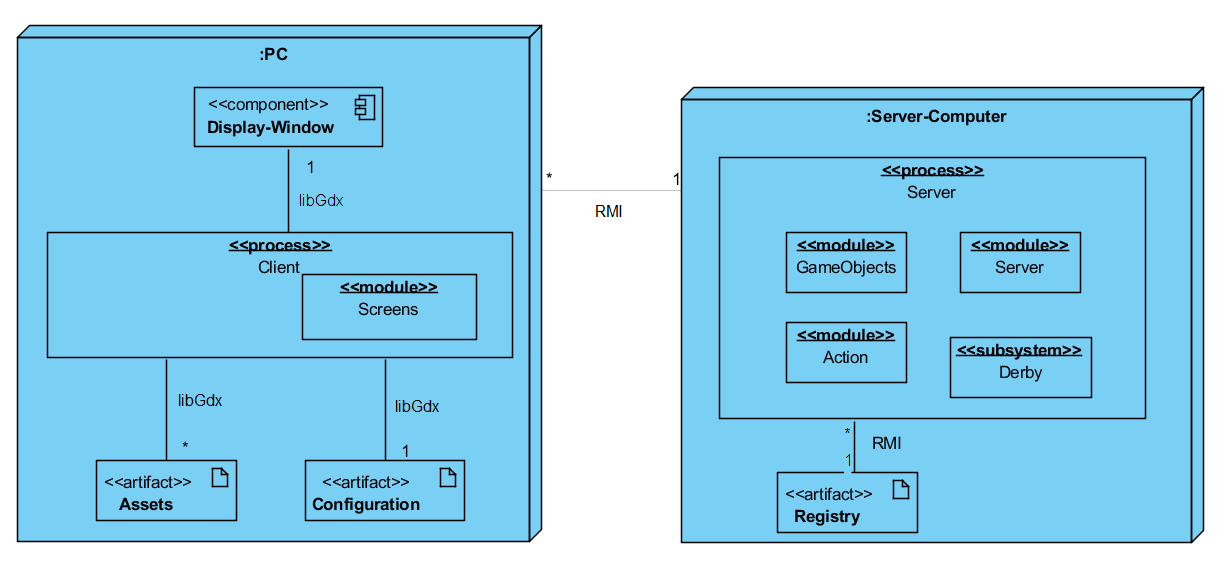
\includegraphics[width=1.0\linewidth]{Deployment}
\caption{Ausführungssicht als Deployment-Diagramm}
\label{fig:Deployment}
\end{figure}

Wie auf dem Diagramm zu sehen, läuft der Client-Prozess auf dem PC des Benutzers. Der Prozess selbst beinhaltet lediglich das Screens-Modul da, wie bereits im Paket-Diagramm der Modulsicht zu sehen war, die Module Assets und Configuration, kein direkter Teil der Implementation sind sondern Dateien auf dem PC. Der Client-Prozess gibt seine Informationen auf einem Fenster als Schnittstelle für den Benutzer aus. Die Verwendung der Assets, Configuration und des Ausgabefensters wird vom libGdx-Framework übernommen. Wie man sieht, findet direkt auf dem Client nur Darstellungsrelevantes statt, wodurch wir die Möglichkeit zum Schummeln für den Client minimieren.

Über RMI kommuniziert der Client mit dem Server-Computer. Auf dem Server-Computer laufen der Server-Prozess und die für RMI benötigte Registry. Dabei liegt immer nur eine Registry gleichzeitig auf dem PC, da RMI keine Verwendung verschiedener Registrys vorsieht und diese daher nicht unterschieden werden könnten. Die Registry kann jedoch von beliebig vielen Clients und Server-Prozessen verwendet werden, was die Strategie mehrere Verbindungen zuzulassen realisiert, außerdem werden Clients dadurch automatisch synchronisiert. Die Registry wird falls nötig vom Server Prozess angelegt. Im Server-Prozess finden sich dann die GameObjects-Module (welche hier zur Übersichtlichkeit zusammengefasst wurden und somit den gleichen Inhalt wie die GameObjects-Komponente aus Kapitel 3 haben), das Action-Modul, sowie das Server-Modul. Das Server-Modul initialisiert das System und die Registry und ermöglicht dadurch den Zugriff für den Client. Danach greift der Client nur noch auf GameObjects zu und falls nötig minimal auf Action. 

Außerdem findet sich in dem Server-Prozess noch die Derby-Datenbank. Diese liegt auf dem Server-Computer, da nach den Anforderungen die Datenbank nicht installiert werden soll, sie muss also direkt vom Programm verwaltet werden und nicht einfach nur eine Verbindung aufbauen.

Zuletzt ist anzumerken, dass die Client- und Server-Prozesse nicht zwangsläufig auf zwei verschiedenen Computern laufen müssen, es ist durchaus möglich, durch die Strategie Client und Server in ein einzelnes Programm zu schreiben, dass beide Systeme auf dem gleichen Computer laufen. In diesem Fall bleiben die Inhalte der Prozesse gleich und auch an den Artefakten bzw. Komponenten ändert sich nichts, die Kommunikation erfolgt weiterhin über RMI, wobei lediglich ''localhost'' als Zielcomputer verwendet wird, umso auf den aktuellen Computer zu verweisen.


\section[Zusammenhänge zwischen Anwendungsfällen und Architektur]{Zusammenhänge zwischen Anwendungsfällen und Architektur\sectionmark{Zusammenhänge AF u. Architektur}}
\sectionmark{Zusammenhänge AF u. Architektur}
\label{sec:anwendungsfaelle}

In diesem Kapitel wird nun der Zusammenhang zwischen Anwendungsfällen und der Architektur mithilfe von Sequenzdiagrammen veranschaulicht. Bei den Diagrammen fällt eventuell auf, dass die Methoden auf Client-Ebene sehr generische Namen besitzen. Dies liegt daran, dass diese, wie bereits in der Modulsicht beschrieben, noch nicht genau definiert sind, die Namen sind daher Repräsentanten für entsprechende Funktionen, wobei es mehrere Variationen dieser Methoden geben kann, abhängig von der speziellen Auswahl, welche in den Beispielen nicht genauer definiert sind. Diese Variationen unterscheiden sich jedoch nur von speziellen Werten und nicht im Ablauf.

\subsection{Erstellen einer Einheit}
\begin{figure}[h]
\centering
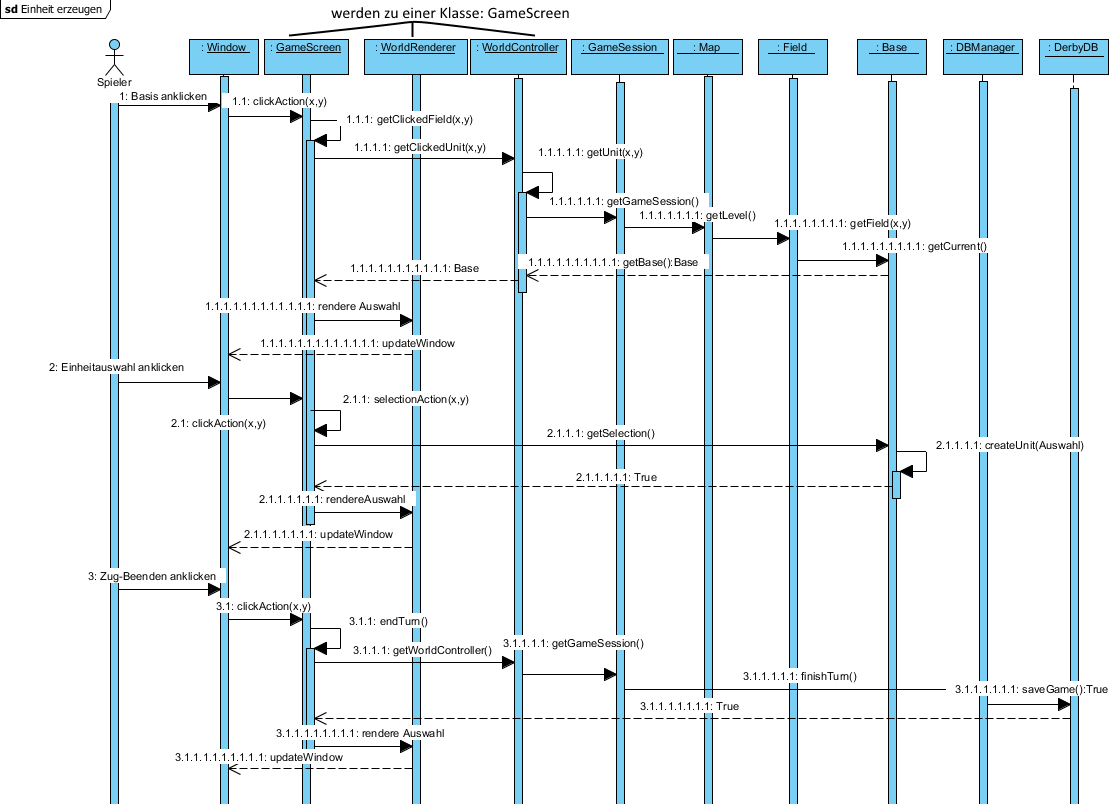
\includegraphics[width=1.0\linewidth]{sequenzdiagramm1}
\caption{Das Erstellen einer Einheit}
\label{fig:sequenzdiagramm1}
\end{figure}

Bei diesem Anwendungsfall möchte der Spieler eine Einheit erstellen und danach seinen Zug beenden.
Er beginnt damit auf eine Basis zu klicken, welche auf seinem Fenster angezeigt wird, um diese aus zu wählen. Dies führt zu einer Kette von Abfragen, welche jeweils ein Element abfragen, um von diesem dann das nächste Element zu erhalten, bis schlussendlich die Basis zurückgegeben wird. Die Anfrage beginnt dabei in GameScreen(bzw. Window) und wird durch WorldRenderer und WorldController an die GameSession übersetzt. Diese leitet die Anfrage dann an ihre Elemente weiter, gemäß der Klassenhierarchie. 

Ist die Frage dann beim Feld angekommen, liefert dieses die Basis zurück, welche bis zum GameScreen durchgereicht wird. Nun haben sich die Informationen des Bildschirms geändert, was beim nächsten Rendern sichtbar wird (das tatsächliche Rendern wird, wie in den vorherigen Kapiteln bereits beschrieben, von libGdx übernommen). Da die Basis nun ausgewählt und diese Auswahl im Fenster dargestellt ist, kann der Spieler nun die Einheitenauswahl anklicken. Dies bewirkt, dass der GameScreen die an die Einheitenauswahl gebundene Funktion ausführt, was in diesem Fall ein Aufrufen von createUnit auf der ausgewählten Basis entspricht. Die Parameter für die Methoden sind dabei durch die spezielle Einheitenauswahl definiert. Innerhalb der createUnit-Methode wird dann überprüft, ob die Methoden ausgeführt werden können. Dieser Prozess ist für den Anwendungsfall nicht von Interesse, da wir davon ausgehen dass alle Bedingungen zum Erstellen der Einheit erfüllt sind, darum betrachten wir diesen Aspekt nicht genauer. Da alle erforderlichen Bedingungen erfüllt sind, gibt die Methode true zurück und die Render-Informationen aktualisieren sich erneut.

Zuletzt wählt der Spieler ''Zug beenden'' aus. Diese Anfrage wird durch den GameScreen weitergeleitet und vom WorldRenderer und WorldController an die GameSession übersetzt. Dort wird dann finishTurn aufgerufen, was das Ende der Runde kennzeichnet und den DBManager anweist die Session zu speichern. Da dieser Prozess in unserem Beispiel erfolgreich ist, wird nun noch true zurück gegeben und die Render-Informationen ein letztes Mal aktualisiert.


\subsection{Einheit wurde bewegt}

\begin{figure}[h]
\centering
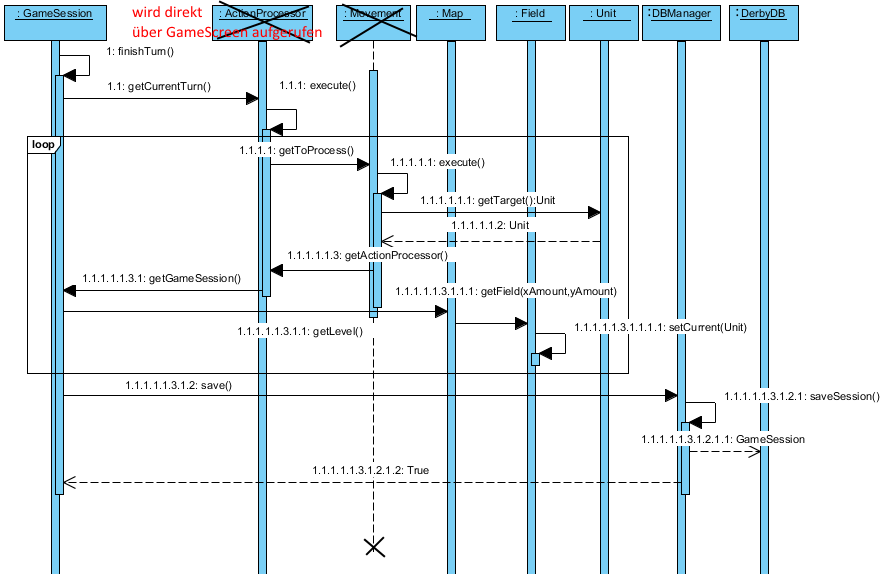
\includegraphics[width=1.0\linewidth]{sequenz2}
\caption{Der Prozess nachdem eine Einheit bewegt wurde}
\label{fig:sequenz2}
\end{figure}

Dieser Anwendungsfall beginnt nachdem eine Einheit bewegt wurde und finishTurn aufgerufen wurde. 

Daraufhin wird im ActionProcessor die execute-Methode aufgerufen, wodurch eine Schleife beginnt, in der für jede Action innerhalb des ActionProcessors execute() ausgeführt wird. In diesem Beispiel ist die einzige existierende Action die Movement-Action. Diese bewegt die Einheit bei ihrer Ausführung auf ein leeres Feld. Wurde diese Methode ausgeführt, wird ein Movement-Objekt nicht weiter verwendet. Sind alle Actions des ActionProcessor-Objektes ausgeführt worden, wird die GameSession in der Datenbank gespeichert. Danach ist der nächste Spieler am Zug.


\section{Evolution}

\label{sec:evolution}

Eine mögliche Änderung wäre der Wechsel von Gradle auf Maven. Dieser hätte für die Architektur selbst keine Auswirkungen, allerdings müssten alle Gradle bezogenen Dateien(z.B. build Dateien) entfernt werden und entsprechende Maven Dateien integriert werden, speziell müssten die Dependencys aus der allgemeinen build.gradle Datei in die pom.xml von Maven übertragen werden.

Würde man von RMI auf TCP/IP Kommunikation wechseln, würde man einige weitere Klassen hinzufügen, welche die Kommunikation ermöglichen und müsste vermutlich jegliche Methodenaufrufe anpassen, also das gesamte System halb neu schreiben.

Eine weitere mögliche Änderung wäre ein Wechsel der Datenbank auf z.B. SQLite. In diesem Fall müsste man lediglich den Inhalt der Klasse DBManager an die jeweilige neue Schnittstelle anpassen, Änderungen an der Architektur wären jedoch nicht möglich, sofern die neue Datenbank keine speziellen Anforderungen an den Aufbau von Objekten hat.

Neben der grafischen Darstellung ist auch eine textliche Darstellung möglich. Ein Wechsel würde keine Änderung in der Architektur benötigen. Stattdessen müsste die Darstellung in den Screenklassen angepasst werden und der Großteil der Assets-Komponente würde wegfallen.

Um die Exzellenz-Anforderungen wie z.B. den Einheiteneditor zu erfüllen muss die Architektur um entsprechende Klassen erweitert werden, welche den Zugriff für den Spieler ermöglichen und die Werte in den Einheiten, die editierbar sein sollen, entsprechend zu manipulieren.

Eine bisher nicht betrachtete Änderung, da sie nicht geplant ist, wäre weitere Statistiken für den Spieler anzulegen. Dafür müsste man das Player- bzw. Account-Objekt um entsprechende Inhalte erweitern und gegebenenfalls zusätzliche Screens zur Betrachtung dieser Statistiken hinzufügen.

Zu guter Letzt ist eine Aufteilung von Server und Client auf zwei Programme denkbar. In diesem Fall müsste man die Server-Komponente auf ein Maven-Projekt auslagern um die Mindestanforderungen weiterhin zu erfüllen. Außerdem müsste man das übrige Client-Programm um die Interfaces der Server-Komponente erweitern, wobei zu beachten ist, dass diese die gleiche Struktur bezüglich der Pakete aufweisen müssen.

\section{Dokumentation}

\label{sec:dokumentation}

Hier werden die Methoden der verschiedenen Klassen dokumentiert, eine Beschreibung der Attribute ist bereits in der Datensicht zu finden. Für die Klassen, welche in der Datensicht als irrelevant betrachtet worden sind, finden sich hier auch Beschreibungen der Attribute. Sollte eine Klasse hier nicht aufgeführt sein, bedeutet das, das sie keine speziellen Methoden besitzt oder diese für die Architektur nicht relevant sind und somit noch nicht genau definiert. Außerdem werden teilweise Hilfsklassen kurz beschrieben, welche zwar der Vollständigkeit halber im Diagramm auftauchen, aber für die restliche Architektur nicht relevant sind. Für eine bessere Orientierung zeigt Abb. 13 noch einmal das gesamte Programm als Klassendiagramm.

Die Dokumentation ist dabei nach Paketen geordnet.

\begin{figure}[h]
\centering
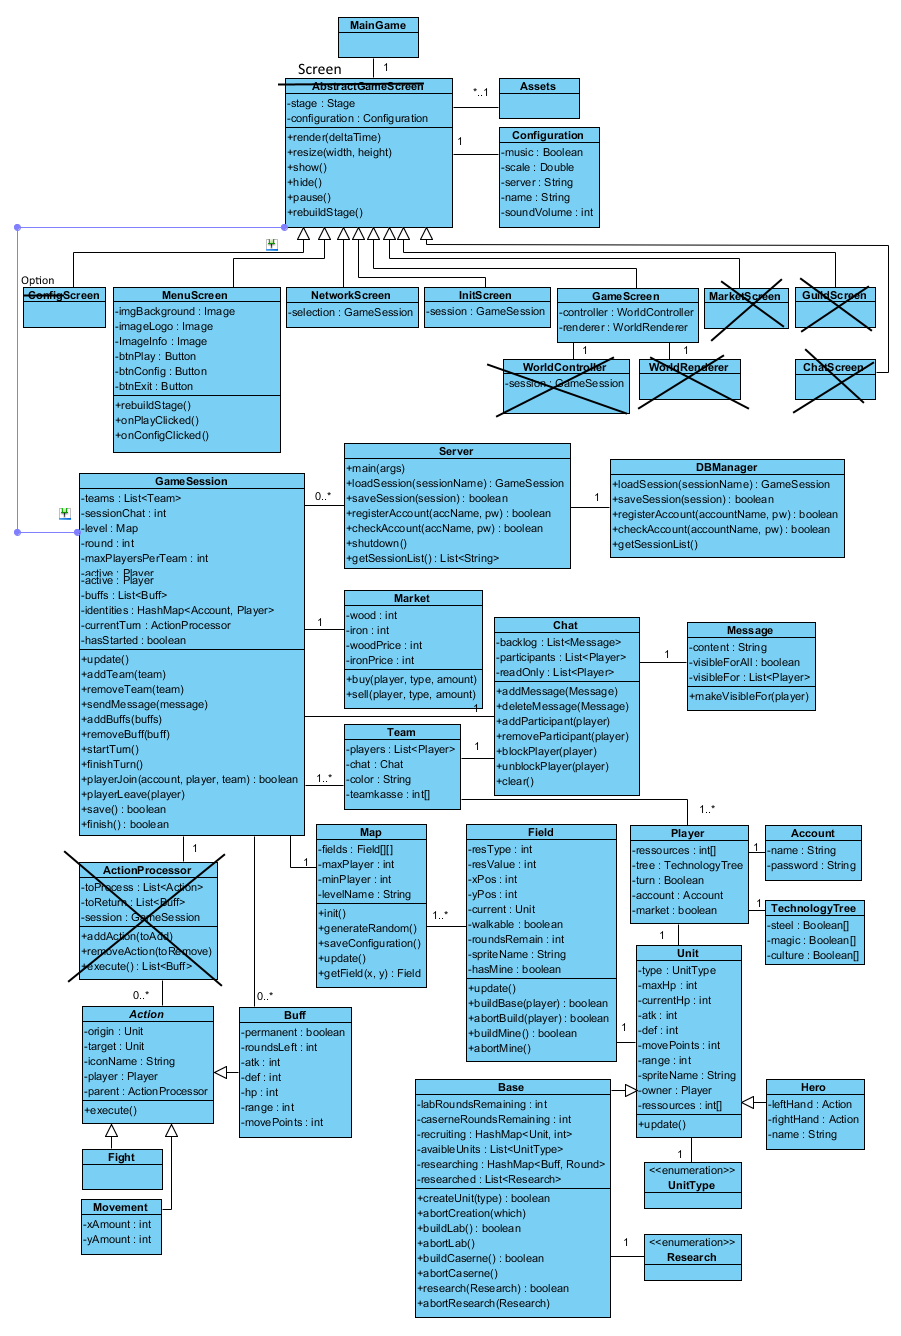
\includegraphics[width=1.0\linewidth]{ClassDiagram1}
\caption{Gold and Greed als Klassendiagramm}
\label{fig:ClassDiagram1}
\end{figure}


\subsection{Screens:}
\subsubsection{AbstractGameScreen}
Diese Klasse stellt das Template dar, welches alle Bildschirme erfüllen müssen. Die Funktionen sind dabei durch das LibGdx-Framework gegeben.\\

\textbf{Attribute:}\\
\begin{itemize}
	\item \textbf{game:} Diese Attribut speichert dass aktuell laufende Programm und dient als Schnittstelle um den Bildschirm zu wechseln.
	\item \textbf{gamesession:} Diese Attribut speichert das aktuelle Spiel und wird verwendet, um auf alle benötigten Informationen des Spiels zuzugreifen. Da das Spiel frühestens im NetworkScreen geladen wird, ist dieses Attribut für alle vorherigen Screens(ConfigScreen und MenuScreen) \textbf{null}.
	\item \textbf{stage:} Dieses Attribut stellt das aktuelle Level des Spiels dar.
	\item \textbf{configuration:} Hier wird das ConfigObjekt gespeichert, wodurch lokale Einstellungen eines Computers abgerufen werden können.
\end{itemize}

\textbf{Methoden:}
\begin{itemize}
	\item \textbf{render:} Die Methoden bestimmen was im nächsten Bild dargestellt wird. Der Parameter ''deltaTime'' wird vom Framework gegeben und gibt die Zeit zum letzten Bild an. Dies wird benötigt, um die Berechnungen Frame-unabhängig zu gestalten. In dieser Methode wird auch auf die Assets zu gegriffen.
	\item \textbf{resize:} Diese Funktion wird verwendet, um die Größe des dargestellten Fensters zu ändern (ausgenommen Vollbild). Die Parameter sind selbsterklärend.
	\item \textbf{show:} Hiermit wird ein Bildschirm aktiv geschaltet.
	\item \textbf{hide:} Diese Methode deaktiviert einen Bildschirm wieder.
	\item \textbf{pause:} Mit dieser Methode kann das Rendern des Spiels pausiert werden und ist durch das Framework gegeben, für Desktop-Applikationen jedoch irrelevant.
	\item \textbf{rebuildStage:} Hiermit kann das Level auf den Ursprungszustand zurückgesetzt werden.
\end{itemize}

\subsubsection{Config:}
\textbf{Methoden:}
\begin{itemize}
	\item \textbf{addServer/removeServer:} Fügt einen Server hinzu oder entfernt einen. Bekommt die IP des Servers als Parameter in Stringform übergeben.
\end{itemize}

\subsubsection{WorldController}

Dies ist eine Hilfsklasse, für die Kontrolle des Spiellevels, welche nach dem Framework verwendet wird, daher keine genauere Erklärung.

\subsubsection{WorldRenderer}

Dies ist eine Hilfsklasse, für die Darstellung des Spiellevels, welche nach dem Framework verwendet wird, daher keine genauere Erklärung.

\subsection{ServerMain:}
\subsubsection{Server:}
\textbf{Methoden:}
\begin{itemize}
	\item \textbf{main:} Initialisiert das System und stellt eine Registry zur Verfügung.
	\item \textbf{loadSession:} Leitet die Anfrage an die gleichnamige DBManager Funktion weiter. Daher siehe DBManager.
	\item \textbf{saveSession:} Leitet die Anfrage an die gleichnamige DBManager Funktion weiter. Daher siehe DBManager.
	\item \textbf{registerAccount:} Leitet die Anfrage an die gleichnamige DBManager Funktion weiter. Daher siehe DBManager.
	\item \textbf{checkAccount:} Leitet die Anfrage an die gleichnamige DBManager Funktion weiter. Daher siehe DBManager.
	\item \textbf{shutdown:} Speichert alle ungespeicherten Spiele und beendet die Registry, sowie den Server.
	\item \textbf{getSessionList:} Liefert eine Liste mit den Namen aller auf dem Server verfügbaren Spielen, unter Verwendung des DBManagers zurück.
	\item \textbf{deleteAccount:} Leitet die Anfrage an die gleichnamige DBManager Funktion weiter. Daher siehe DBManager.
	\item \textbf{deleteSession:} Leitet die Anfrage an die gleichnamige DBManager Funktion weiter. Daher siehe DBManager.
\end{itemize}


\subsubsection{DBManager:}
\textbf{Methoden:}
\begin{itemize}
	\item \textbf{loadSession:} Lädt das Spiel mit dem übergebenen Namen aus der Datenbank und gibt es zurück. Falls kein passendes Spiel existiert, wird \textbf{null} zurückgegeben.
	\item \textbf{saveSession:} Speichert das übergebene Spiel in der Datenbank. Rückgabewert gibt an, ob das Speichern funktioniert hat.
	\item \textbf{registerAccount:} Speichert einen neuen Account mit dem übergebenen Namen und Passwort in der Datenbank. Rückgabewert gibt an, ob der Vorgang erfolgreich war.
	\item \textbf{checkAccount:} Überprüft die übergebenen Werte auf einen korrekten Account in der Datenbank. Rückgabewert gibt an ob, die Werte korrekt sind oder nicht.
	\item \textbf{deleteAccount:} Löscht den angegebenen Account aus der Datenbank, sofern er existiert, sonst passiert nichts.
	\item \textbf{deleteSession:} Löscht die GameSession aus der Datenbank, sofern sie existiert, sonst passiert nichts.
\end{itemize}


\subsection{GameObject:}
\subsubsection{GameSession:}
\textbf{Methoden:}
\begin{itemize}
	\item \textbf{update:} Fordert alle Objekte des Spiels auf sich zu aktualisieren.
	\item \textbf{addTeam:} Fügt ''teams'' das übergebene Objekt hinzu.
	\item \textbf{removeTeam:} Entfernt das übergebene Team aus ''teams'', wenn es nicht vorhanden ist passiert nichts.
	\item \textbf{sendMessage:} Fügt dem Spielchat die übergebene Nachricht hinzu.
	\item \textbf{addBuffs:} Fügt eine Liste von Buffs zu ''buffs'' hinzu. Wird nur von ActionProcessor verwendet.
	\item \textbf{removeBuff:} Analog zu ''removeTeam'' für ''buffs''.
	\item \textbf{startTurn:} Initialisiert den nächsten Zug, d.h. wechselt den aktiven Player.
	\item \textbf{finishTurn:} Beendet den aktuellen Zug, d.h. fordert den ActionProcessor auf seine Inhalte zu verarbeiten, speichert alle Änderungen und ruft startTurn auf.
	\item \textbf{playerJoin:} Fügt einen neuen Spieler mit dem übergebenen Account zu dem übergebenen Team hinzu(sowie zu identities). Rückgabewert gibt an ob der Vorgang erfolgreich war.
	\item \textbf{playerLeave:} Entfernt den übergebenen Spieler aus dem Spiel und damit auch alle zugehörigen Objekte.
	\item \textbf{save:} Weist den Server an die Sitzung zu speichern. Rückgabewert gibt an, ob der Vorgang erfolgreich war.
	\item \textbf{finish:} Beendet das Spiel. Es wird nicht beachtet ob das Spiel gespeichert ist. Gibt es einen Sieger wird dies angegeben und das Spiel danach gelöscht. Rückgabewert gibt an, ob der Vorgang erfolgreich war.
	\item \textbf{createAction:} Dient zum Erstellen einer neuen Action, so dass das Action-Interface nur für die Funktionalität benötigt wird. Der erste Paramter gibt an, um was für eine Action es sich handeln soll (z.B. ''Fight''). Die weiteren Parameter entsprechen den Grundattributen einer Action. Alle spezifischeren Attribute werden danach über die setter gesetzt. Der Rückgabewert entspricht der erstellen Action.
\end{itemize}

\subsubsection{Map:}
\textbf{Methoden:}
\begin{itemize}
	\item \textbf{init:} Diese Methode generiert die Felder der Karte, sowie max/minPlayer. Zu Beginn wird eine Karte Hard-gecoded. Wenn im Laufe des Projektes genügend Zeit übrig ist, werden Karten in Dateien gespeichert und bei init ausgelesen, wobei die Datei über ''levelName'' identifiziert wird.
	\item \textbf{generateRandom:} Generiert eine zufällige Karte. Wird nur bei genug übriger Zeit des Projektes implementiert.
	\item \textbf{saveConfiguration:} Speichert die Karte in einer Datei, wird erst implementiert wenn genug Zeit im Projektverlauf übrig ist.
	\item \textbf{update:} Fordert alle Felder dazu auf sich zu aktualisieren.
	\item \textbf{getField:} Gibt das Feld mit den Koordinaten X und Y zurück.
\end{itemize}

\subsubsection{Unit:}
\textbf{Methoden:}
\begin{itemize}
	\item \textbf{update:} Aktualisiert die Einheit, derzeit nur für Base nötig, später jedoch eventuell noch für andere.
\end{itemize}


\subsubsection{Base:}
\textbf{Methoden:}
\begin{itemize}
	\item \textbf{createUnit:} Rekrutiert eine Einheit des übergebenen Typs. Rückgabewert gibt an, ob der Vorgang erfolgreich war.
	\item \textbf{abortCreation:} Bricht den Rekrutierungsvorgang der übergebenen Einheit ab, sofern vorhanden. Analog zu ''abortBuild'' von Field.
	\item \textbf{buildLab:} Startet den Bau des Labors. Rückgabewert gibt an ob der Vorgang erfolgreich war.
	\item \textbf{abortLab:} Analog zu ''abortCreation'' für das Labor(wobei es immer nur ein Labor-Bauauftrag geben kann, daher kein Parameter).
	\item \textbf{buildCaserne:} Analog zu ''buildLab'' für die Kaserne.
	\item \textbf{abortCaserne:} Analog zu ''abortLab'' für die Kaserne.
	\item \textbf{research:} Erforscht die übergebene Forschung bzw. Verbesserung. Rückgabewert gibt an, ob der Vorgang erfolgreich war.
	\item \textbf{abortResearch:} Bricht den Forschungsauftrag der übergebenen Forschung ab, wenn vorhanden, sonst passiert nichts.
\end{itemize}

\subsubsection{Market:}
\textbf{Methoden:}
\begin{itemize}
	\item \textbf{buy:} Lässt den angegebenen Spieler die angegebene Menge Holz oder Eisen kaufen. Type bestimmt ob Holz oder Eisen (0=Holz, 1=Eisen). Kein Rückgabewert, die Werte werden direkt manipuliert. Zuletzt wird der jeweilige Preis neu berechnet in Abhängigkeit von einem Standardwert und der vorhandenen Menge.
	\item \textbf{sell:} Analog zu ''buy'', nur dass hier die Ressourcen verkauft und nicht gekauft werden.
\end{itemize}

\subsection{Action:}
\subsubsection{ActionProcessor}:
\textbf{Methoden:}
\begin{itemize}
	\item \textbf{addAction:} Fügt die übergebene Action zu ''toProcess'' hinzu.
	\item \textbf{removeAction:} Entfernt die übergeben Action aus ''toProcess'', sofern vorhanden, ansonsten passiert nichts.
	\item \textbf{execute:} Führt alle Actions in toProcess aus und überprüft ob sich dadurch neue Actions oder Buffs ergeben. Neue Actions werden ebenfalls ausgeführt, Buffs werden zu ''toReturn'' hinzu gefügt. Am Ende wird ''toReturn'' zurückgegeben, damit die Buffs in der GameSession gespeichert werden können.
\end{itemize}

\subsubsection{Action:}
\textbf{Methoden:}
\begin{itemize}
	\item \textbf{execute:} Führt die Aktion aus. Konkreter Inhalt ist von den jeweiligen Aktionen abhängig.
\end{itemize}



\subsection{Chat:}
\subsubsection{Chat(Klasse):}
\textbf{Methoden:}
\begin{itemize}
	\item \textbf{addMessage:} Fügt die übergebene Nachricht zu ''backlog'' hinzu.
	\item \textbf{removeMessage:} Entfernt die übergebene Nachricht aus ''backlog'', sofern vorhanden, ansonsten passiert nichts.
	\item \textbf{addParticipant:} Analog zu addMessage für ''participants''.
	\item \textbf{removeParticipant:} Analog zu removeMessage für ''participants''.
	\item \textbf{blockPlayer:} Verschiebt den angegebenen Spieler von ''participants'' zu ''readOnly''. Ist der Spieler nicht vorhanden oder bereits in ''readOnly'' passiert nichts.
	\item \textbf{unblockPlayer:} Analog zu blockPlayer in umgekehrter Richtung(also ''readOnly'' zu ''participants'').
	\item \textbf{clear:} Leert den backlog des Chat.
\end{itemize}

\subsubsection{Message:}
\textbf{Methoden:}
\begin{itemize}
	\item \textbf{makeVisibleFor:} Fügt einen Spieler zu ''visibleFor'' hinzu und ermöglicht ihm so die Nachricht zu lesen. Der Vorgang kann nicht rückgängig gemacht werden.
\end{itemize}



\end{document}








%%% Local Variables: 
%%% mode: latex
%%% mode: reftex
%%% mode: flyspell
%%% ispell-local-dictionary: "de_DE"
%%% TeX-master: t
%%% End: 
